\documentclass[
  12pt,
  oneside,
  a4paper,
  sumario=tradicional,
  brazil
]{abntex2}

\setlrmarginsandblock{3cm}{2cm}{*}
\setulmarginsandblock{3cm}{2cm}{*}
\checkandfixthelayout

\usepackage{fontspec}
\usepackage{graphicx}
\usepackage{enumitem}
\usepackage{ragged2e}
\usepackage{xurl}
\usepackage{amsmath}
\usepackage{float}
\usepackage{tikz}
\usetikzlibrary{arrows.meta, positioning, shapes.geometric, calc}
\usepackage{microtype}
\usepackage{array}
\usepackage{booktabs}
\usepackage{tabularx}
\usepackage{longtable}
\usepackage[table]{xcolor}
\usepackage{csquotes}
\usepackage[backend=biber,style=abnt]{biblatex}
\addbibresource{refs.bib}

\defaultfontfeatures{Ligatures=TeX}
\IfFontExistsTF{Times New Roman}
  {\setmainfont{Times New Roman}}
  {\setmainfont{Liberation Serif}}
\urlstyle{same}

\setlength{\parindent}{1.3cm}
\setlength{\parskip}{0pt}
\setlength{\emergencystretch}{3em}

\newcommand{\bodyfont}{\fontsize{12}{18}\selectfont}
\newcommand{\coverfont}{\fontsize{14}{21}\selectfont}
\newcommand{\smallfontdoc}{\fontsize{10}{12}\selectfont}
\newcolumntype{P}[1]{>{\RaggedRight\arraybackslash}p{#1}}
\newcolumntype{Y}{>{\RaggedRight\arraybackslash}X}
\newcolumntype{C}[1]{>{\centering\arraybackslash}p{#1}}
\newcommand{\timeline}{\(\bullet\)}
\definecolor{pequiDark}{HTML}{2F4F1F}
\definecolor{pequiGreen}{HTML}{6F8F2F}
\definecolor{pequiLeaf}{HTML}{4F772D}
\definecolor{pequiLight}{HTML}{EEF6D8}
\definecolor{pequiPulp}{HTML}{F2C94C}
\definecolor{pequiPulpLight}{HTML}{FFF4C2}
\definecolor{pequiEarth}{HTML}{A65F2B}
\definecolor{pequiBlue}{HTML}{BFDDE0}
\definecolor{tablehead}{HTML}{EEF6D8}
\definecolor{tablerule}{HTML}{2F4F1F}
\definecolor{tableaccent}{HTML}{6F8F2F}
\arrayrulecolor{tablerule}
\setlength{\heavyrulewidth}{0.8pt}
\setlength{\lightrulewidth}{0.45pt}

\titulo{Orquestra\c{c}\~ao din\^amica de filas de caminh\~oes em p\'atios agroindustriais com despacho online sob restri\c{c}\~oes}
\autor{Marcus Vinicius Santos da Silva}
\local{Goi\^ania}
\data{2026}
\instituicao{Pontif\'icia Universidade Cat\'olica de Goi\'as\par Escola Polit\'ecnica e de Artes\par Gradua\c{c}\~ao em Ci\^encia da Computa\c{c}\~ao}
\tipotrabalho{Trabalho de Conclus\~ao de Curso I}
\preambulo{Trabalho de Conclus\~ao de Curso I apresentado ao curso de Ci\^encia da Computa\c{c}\~ao da Pontif\'icia Universidade Cat\'olica de Goi\'as, como requisito acad\^emico parcial para a conclus\~ao da gradua\c{c}\~ao.}
\orientador{Profa. Dra. Maria Jos\'e Dantas}

\makeatletter
\hypersetup{
  pdftitle={\@title},
  pdfauthor={\@author},
  pdfsubject={\imprimirpreambulo},
  pdfcreator={LaTeX with abnTeX2},
  pdfkeywords={despacho online, p\'atios agroindustriais, simula\c{c}\~ao de eventos discretos, sistemas de apoio \`a decis\~ao},
  hidelinks,
  pdfborder={0 0 0},
  pageanchor=true,
  hypertexnames=false,
  bookmarksdepth=4
}
\makeatother

\begin{document}
\selectlanguage{brazil}
\frenchspacing
\pretextual

\begin{titlingpage}
  \centering
  \coverfont
  PONTIF\'ICIA UNIVERSIDADE CAT\'OLICA DE GOI\'AS\par
  ESCOLA POLIT\'ECNICA E DE ARTES\par
  GRADUA\c{C}\~AO EM CI\^ENCIAS DA COMPUTA\c{C}\~AO\par

  \vspace{4.4cm}
  
\includegraphics[width=6.53cm]{images/puc-goias.png}\par

  \vspace{3.6cm}
  {\bfseries
  ORQUESTRA\c{C}\~AO DIN\^AMICA DE FILAS DE\par
  CAMINH\~OES EM P\'ATIOS AGROINDUSTRIAIS COM DESPACHO\par
  ONLINE SOB RESTRI\c{C}\~OES\par}

  \vfill
  \bodyfont
  MARCUS VINICIUS SANTOS DA SILVA\par

  \vfill
  GOI\^ANIA\par
  2026\par
\end{titlingpage}

\begin{titlingpage}
  \centering
  \bodyfont
  \vspace*{0.8cm}
  MARCUS VINICIUS SANTOS DA SILVA\par

  \vspace{9.6cm}
  {\coverfont\bfseries
  ORQUESTRA\c{C}\~AO DIN\^AMICA DE FILAS DE\par
  CAMINH\~OES EM P\'ATIOS AGROINDUSTRIAIS COM DESPACHO\par
  ONLINE SOB RESTRI\c{C}\~OES\par}

  \vspace{2.0cm}
  \hfill
  \begin{minipage}{8.35cm}
    \justifying
    \SingleSpacing
    \smallfontdoc
    Trabalho de Conclus\~ao de Curso I apresentado ao curso de Ci\^encia da Computa\c{c}\~ao da Pontif\'icia Universidade Cat\'olica de Goi\'as, como requisito acad\^emico parcial para a conclus\~ao da gradua\c{c}\~ao.

    \vspace{0.8cm}
    Orientadora: Profa. Dra. Maria Jos\'e Dantas
  \end{minipage}

  \vfill
  GOI\^ANIA\par
  \vspace{0.7cm}
  2026\par

\end{titlingpage}

\begin{folhadeaprovacao}
  \centering
  {\bodyfont MARCUS VINICIUS SANTOS DA SILVA\par}

  \vspace*{2.5cm}
  {\coverfont\bfseries ORQUESTRA\c{C}\~AO DIN\^AMICA DE FILAS DE CAMINH\~OES EM P\'ATIOS AGROINDUSTRIAIS COM DESPACHO ONLINE SOB RESTRI\c{C}\~OES\par}

  \vspace*{2.0cm}
  \hfill
  \begin{minipage}{8.35cm}
    \justifying
    \SingleSpacing
    \smallfontdoc
    Trabalho de Conclus\~ao de Curso I apresentado ao curso de Ci\^encia da Computa\c{c}\~ao da Pontif\'icia Universidade Cat\'olica de Goi\'as, como requisito acad\^emico parcial para a conclus\~ao da gradua\c{c}\~ao.
  \end{minipage}

  \vspace*{1.8cm}
  Aprovado em: \underline{\hspace{1.2cm}}/\underline{\hspace{1.2cm}}/\underline{\hspace{1.8cm}}

  \vspace*{1.5cm}
  \begin{center}
    \rule{10cm}{0.4pt}\par
    Profa. Dra. Maria Jos\'e Dantas\par
    Orientadora -- Pontif\'icia Universidade Cat\'olica de Goi\'as

    \vspace{1.2cm}
    \rule{10cm}{0.4pt}\par
    Membro da banca examinadora

    \vspace{1.2cm}
    \rule{10cm}{0.4pt}\par
    Membro da banca examinadora
  \end{center}
\end{folhadeaprovacao}

\begin{resumo}
  P\'atios de recebimento de gr\~aos enfrentam congestionamentos durante o pico de safra
  decorrentes da disputa por recursos compartilhados --- balan\c{c}as, moegas e \'areas de
  espera. Pol\'iticas est\'aticas de fila amplificam esses atrasos ao n\~ao reagir a eventos
  disruptivos como chuva, falhas de equipamento, bloqueios documentais e mudan\c{c}as de
  prioridade contratual. Este trabalho prop\~oe e especifica um motor de apoio \`a decis\~ao
  para a orquestra\c{c}\~ao din\^amica de caminh\~oes em p\'atios agroindustriais, formulado
  como problema de \textbf{despacho online sob restri\c{c}\~oes} com reavalia\c{c}\~ao
  cont\'inua do estado operacional. O motor combina filtro de factibilidade por
  restri\c{c}\~oes r\'igidas, ranqueamento lexicogr\'afico local com horizonte curto e
  registro audit\'avel de cada decis\~ao, preservando a supervis\~ao humana. A metodologia
  adotada \'e o Design Science Research, com desenvolvimento e avalia\c{c}\~ao de artefato
  computacional em cen\'arios sint\'eticos controlados via simula\c{c}\~ao de eventos
  discretos. A compara\c{c}\~ao ser\'a pareada contra quatro pol\'iticas de refer\^encia ---
  FIFO estrito, FIFO \textit{flow-faithful}, prioridade com factibilidade local e despacho
  por escore fixo --- sob configura\c{c}\~oes de carga baixa, m\'edia e alta congest\~ao,
  com eventos disruptivos. A hip\'otese central (H1) prev\^e redu\c{c}\~ao de pelo menos
  15\% no p95 da espera acumulada em fila nos estratos de m\'edia e alta congest\~ao, sem
  perda de throughput mediano acima da margem protetiva definida por escala. Dois crit\'erios de aceita\c{c}\~ao
  de engenharia complementam H1: taxa nula de viola\c{c}\~ao de restri\c{c}\~oes r\'igidas
  (A1) e rastreabilidade integral das decis\~oes e interven\c{c}\~oes humanas (A2). Esta
  etapa (TCC~I) entrega a modelagem formal, o protocolo experimental completo, os artefatos
  preliminares de reprodutibilidade e os comparadores congelados; a execu\c{c}\~ao dos experimentos
  comparativos \'e prevista para o TCC~II. Como camada de representa\c{c}\~ao, ser\'a
  desenvolvido no Unreal Engine~5.8 um \textbf{modelo digital} tridimensional do p\'atio,
  alimentado por exporta\c{c}\~oes e replays do simulador. O termo g\^emeo digital n\~ao \'e
  adotado, pois n\~ao existe, nesta etapa, um ativo f\'isico individual pareado nem
  sincroniza\c{c}\~ao bidirecional em tempo real.

  \vspace{\onelineskip}
  \noindent
  \textbf{Palavras-chave}: despacho online. p\'atios agroindustriais. simula\c{c}\~ao de
  eventos discretos. modelo digital. Unreal Engine. sistemas de apoio \`a decis\~ao.
  \textit{scheduling} sob incerteza.
\end{resumo}

\begin{resumo}[Abstract]
  Grain receiving yards face congestion during harvest peaks due to competition for shared
  resources such as scales, hoppers and waiting areas. Static queue policies may intensify
  delays when they do not react to rain, equipment failures, document blocks and contractual
  priority changes. This work proposes and specifies a decision-support engine for the dynamic
  orchestration of trucks in agro-industrial yards, formulated as an online constrained
  dispatching problem with continuous reassessment of the operational state. The engine combines
  a feasibility filter for hard constraints, local lexicographic ranking with a short horizon and
  auditable records for each decision while preserving human supervision. The methodology follows
  Design Science Research, with the development and evaluation of a computational artifact in
  controlled synthetic scenarios through discrete-event simulation. The comparison will use
  FIFO strict, FIFO \textit{flow-faithful}, priority with local feasibility and fixed-score
  dispatching as reference policies under low-load, medium-congestion and high-congestion
  configurations with disruptive events. The central hypothesis (H1) predicts at least a
  15\% reduction in the paired median p95 of accumulated queue waiting time in the medium-
  and high-congestion families, without median throughput loss above the scale-adjusted
  protective margin. Two engineering acceptance criteria complement H1: no violation of hard
  constraints (A1) and full traceability of decisions and human interventions (A2). This
  TCC~I stage delivers the formal model, the experimental protocol, preliminary
  reproducibility artifacts and frozen comparators; the main comparative experiments are
  planned for TCC~II. A three-dimensional \textbf{digital model} of the yard will be
  developed in Unreal Engine~5.8 as a representation layer fed by simulator exports and
  replays. The term digital twin is not used because this stage has neither a paired
  individual physical asset nor real-time bidirectional synchronization.

  \vspace{\onelineskip}
  {\RaggedRight
  \textbf{Keywords}: online dispatching. agro-industrial yards.
  discrete-event simulation. digital model. Unreal Engine. decision-support systems.
  scheduling under uncertainty.
  \par}
\end{resumo}

\pdfbookmark[0]{Lista de ilustra\c{c}\~oes}{lof}
\listoffigures*
\cleardoublepage

\pdfbookmark[0]{Lista de tabelas}{lot}
\listoftables*
\cleardoublepage

\pdfbookmark[0]{\contentsname}{toc}
\tableofcontents*
\cleardoublepage

\textual
\OnehalfSpacing

\chapter{Introdução}

P\'atios de recebimento de gr\~aos concentram, em janelas de pico, fluxos de caminh\~oes que disputam portarias, balan\c{c}as, moegas e \'areas de espera. Quando a opera\c{c}\~ao combina alta variabilidade, recursos heterog\^eneos e restri\c{c}\~oes simult\^aneas, pol\'iticas est\'aticas tendem a perder ader\^encia ao estado real do p\'atio. Esse problema j\'a aparece na literatura de agendamento de caminh\~oes e congestionamento em terminais \parencite{abdelmagidComprehensiveReviewTruck2022a, graciaTruckAppointmentScheduling2025a}; aqui, ele \'e tratado no recorte espec\'ifico do recebimento agroindustrial.

A dificuldade n\~ao est\'a apenas em ordenar uma fila. Atrasos, falhas, chuva, bloqueios documentais e mudan\c{c}as de prioridade podem tornar uma sequ\^encia planejada obsoleta em poucos eventos. Por isso, este trabalho parte da literatura de scheduling sob incerteza e despacho em tempo real, que recomenda reavalia\c{c}\~ao do plano quando o estado operacional muda \parencite{liProcessSchedulingUncertainty2008a, torbaliMultiagentbasedRealtimeTruck2023}.

No contexto agroindustrial, essa decis\~ao fica mais restrita. Cooperativas e armaz\'ens lidam com sazonalidade intensa, cargas heterog\^eneas, prioridades contratuais, bloqueios documentais, eventos clim\'aticos e exig\^encias de rastreabilidade. Estudos sobre elevadores e terminais graneleiros mostram que recebimento, descarga e mistura de cargas precisam ser modelados com aten\c{c}\~ao ao fluxo f\'isico \parencite{r.berrutoAnalyzingReceivingOperation2001a, turnerDiscreteEventSimulation2019a}. A lacuna explorada aqui est\'a na decis\~ao local de despacho: escolher o pr\'oximo caminh\~ao fact\'ivel quando um recurso fica livre, preservando restri\c{c}\~oes r\'igidas, justificativa e possibilidade de interven\c{c}\~ao humana.

Este trabalho prop\~oe um mecanismo de apoio \`a decis\~ao para orquestrar caminh\~oes em p\'atios agroindustriais como \textbf{despacho online sob restri\c{c}\~oes}. O mecanismo filtra alternativas invi\'aveis, ranqueia candidatos fact\'iveis e registra a recomenda\c{c}\~ao emitida ao operador. A avalia\c{c}\~ao prevista compara o artefato com regras est\'aticas, incluindo FIFO, e com comparadores din\^amicos plaus\'iveis, em cen\'arios simulados com eventos disruptivos.

O problema de pesquisa pode ser formulado nos seguintes termos: como modelar e avaliar um mecanismo de despacho online de caminh\~oes em p\'atios de recebimento de gr\~aos, compar\'avel a regras est\'aticas como FIFO e a comparadores din\^amicos plaus\'iveis, em cen\'arios com m\'ultiplas restri\c{c}\~oes operacionais, mantendo justificativa leg\'ivel, rastreabilidade e possibilidade de interven\c{c}\~ao humana? A formula\c{c}\~ao preserva o foco operacional da decis\~ao: escolher o pr\'oximo atendimento fact\'ivel quando um recurso fica dispon\'ivel e o estado observ\'avel do p\'atio muda.

A pesquisa contribui ao transformar uma decis\~ao operacional recorrente, muitas vezes t\'acita, em um objeto computacional model\'avel e avali\'avel. O enquadramento segue Design Science Research, pois o resultado esperado \'e um artefato verific\'avel, n\~ao apenas uma descri\c{c}\~ao do processo \parencite{hevnerDesignScienceInformation2004a, peffersDesignScienceResearch2007aa}. No plano operacional, a contribui\c{c}\~ao n\~ao \'e automatizar o p\'atio, mas especificar uma recomenda\c{c}\~ao rastre\'avel para atendimentos sob restri\c{c}\~oes duras. Neste texto, \textbf{rastreabilidade} \'e o registro completo da decis\~ao; \textbf{auditabilidade}, a possibilidade de reconstru\c{c}\~ao posterior; \textbf{justificativa leg\'ivel}, a explica\c{c}\~ao compreens\'ivel da regra acionada; e \textbf{governan\c{c}a}, o controle humano autorizado dentro das restri\c{c}\~oes r\'igidas.

Neste trabalho, \textbf{modelo digital} designa a representa\c{c}\~ao computacional do p\'atio
e de seus estados simulados. Essa representa\c{c}\~ao ser\'a produzida no Unreal Engine~5.8
para visualiza\c{c}\~ao tridimensional e replay de eventos, enquanto o simulador de eventos
discretos permanece a fonte das transi\c{c}\~oes e das m\'etricas experimentais. A
classifica\c{c}\~ao como \textbf{g\^emeo digital} seria inadequada: a literatura distingue
modelo, sombra e g\^emeo pelo fluxo de dados entre entidade f\'isica e digital, e as
defini\c{c}\~oes t\'ecnicas atuais exigem conex\~ao e sincroniza\c{c}\~ao com uma contraparte
f\'isica identificada \parencite{kritzingerDigitalTwinManufacturing2018,nistDigitalTwinsEssentialElements2026,isoSmartManufacturingWhitePaper2021}.

\section{Objetivos}

\subsection{Objetivo geral}
Projetar e avaliar um artefato computacional, no contexto estudado, para apoio \`a decis\~ao na orquestra\c{c}\~ao din\^amica de filas de caminh\~oes em p\'atios agroindustriais, visando reduzir tempo de espera, preservar throughput dentro de margem protetiva, acompanhar o uso de recursos e emiss\~oes estimadas de $\mathrm{CO_2}$ como m\'etricas secund\'arias, e manter rastreabilidade das decis\~oes.

\subsection{Objetivos específicos}
\begin{enumerate}[leftmargin=1.27cm,itemsep=0pt,topsep=0pt,parsep=0pt,partopsep=0pt]
  \item Modelar formalmente o problema de p\'atio como um problema de despacho online sob restri\c{c}\~oes.
  \item Definir vari\'aveis, restri\c{c}\~oes r\'igidas e crit\'erios de decis\~ao coerentes com a opera\c{c}\~ao real.
  \item Especificar o motor de decis\~ao proposto, incluindo filtro de factibilidade, regra de ranking e registro audit\'avel.
  \item Construir um prot\'otipo inicial do motor de decis\~ao e seu ambiente de simula\c{c}\~ao.
  \item Desenvolver no Unreal Engine~5.8 um modelo digital tridimensional do p\'atio para visualiza\c{c}\~ao e replay dos estados produzidos pelo simulador.
  \item Comparar o comportamento do motor com pol\'iticas de refer\^encia est\'aticas e din\^amicas plaus\'iveis.
  \item Avaliar o artefato com m\'etricas de espera, throughput, makespan, estabilidade, auditabilidade da decis\~ao e estimativa explorat\'oria de emiss\~oes de $\mathrm{CO_2}$ por marcha lenta.
  \item Discutir riscos operacionais, limites da modelagem e condi\c{c}\~oes de ado\c{c}\~ao pr\'atica.
\end{enumerate}

\section{Hipótese central}

Uma abordagem de orquestra\c{c}\~ao din\^amica baseada em despacho online sob restri\c{c}\~oes ser\'a avaliada por desempenho operacional em cen\'arios com eventos disruptivos e recursos heterog\^eneos, preservando supervis\~ao humana. A avalia\c{c}\~ao separa desempenho comparativo, seguran\c{c}a operacional e governan\c{c}a para evitar que ganhos de fila sejam confundidos com viola\c{c}\~ao de restri\c{c}\~oes ou perda de rastreabilidade. A pesquisa distingue uma hip\'otese comparativa e dois crit\'erios de aceita\c{c}\~ao de engenharia:
\begin{itemize}[leftmargin=1.27cm,itemsep=0pt,topsep=0pt,parsep=0pt,partopsep=0pt]
  \item \textbf{H1 -- desempenho comparativo:} no protocolo comparativo proposto, o motor reduz em pelo menos 15\% a mediana pareada do p95 da espera acumulada em fila frente a cada comparador operacional prim\'ario, nos estratos de m\'edia e alta congest\~ao analisados separadamente; em cada estrato, a decis\~ao \'e conjuntiva e s\'o passa se todos os comparadores prim\'arios tamb\'em respeitarem a margem protetiva de throughput;
  \item \textbf{A1 -- crit\'erio de seguran\c{c}a operacional:} no artefato proposto, nenhuma recomenda\c{c}\~ao final confirmada pelo sistema viola as restri\c{c}\~oes r\'igidas definidas no protocolo;
  \item \textbf{A2 -- crit\'erio de governan\c{c}a:} no artefato proposto, toda recomenda\c{c}\~ao e toda interven\c{c}\~ao humana devem ter justificativa leg\'ivel, registro audit\'avel e rastreabilidade suficiente para reconstru\c{c}\~ao posterior.
\end{itemize}
Somente \textbf{H1} ser\'a tratada como hip\'otese comparativa entre pol\'iticas. Os crit\'erios \textbf{A1} e \textbf{A2} funcionam como balizadores bin\'arios de aceita\c{c}\~ao do artefato, verificados por log e por auditoria independente, e n\~ao usados para alegar superioridade cient\'ifica sobre as pol\'iticas de refer\^encia. Os limiares quantitativos de H1, A1 e A2 s\~ao detalhados no Cap\'itulo~\ref{ch:metodologia}.

\section{Organização do trabalho}

Este trabalho est\'a organizado em sete cap\'itulos. O Cap\'itulo~2 apresenta o referencial te\'orico. O Cap\'itulo~3 integra metodologia e desenho experimental, reunindo arquitetura do motor, formula\c{c}\~ao alg\'ebrica da heur\'istica lexicogr\'afica, configura\c{c}\~ao do simulador, m\'etricas e pol\'iticas de compara\c{c}\~ao. O Cap\'itulo~4 re\'une os resultados parciais. O Cap\'itulo~5 apresenta o cronograma do TCC~II. O Cap\'itulo~6 discute amea\c{c}as \`a validade e o Cap\'itulo~7 conclui o trabalho. Os ap\^endices documentam pol\'iticas de sensibilidade e materiais contextuais n\~ao confirmat\'orios.

\chapter{Referencial Teórico}\label{ch:referencial}
A base te\'orica parte de uma premissa simples: o recebimento de gr\~aos n\~ao \'e apenas uma fila, mas uma decis\~ao recorrente sob recursos limitados, restri\c{c}\~oes duras e perturba\c{c}\~oes. A primeira literatura mobilizada \'e a de truck appointment systems e coordena\c{c}\~ao de p\'atios. Revis\~oes recentes mostram que a opera\c{c}\~ao envolve sequenciamento, janelas, compatibilidade carga--recurso e controle de congestionamento; uma fila cronol\'ogica simples n\~ao representa esse conjunto de decis\~oes \parencite{abdelmagidComprehensiveReviewTruck2022a, graciaTruckAppointmentScheduling2025a}. Modelos mais recentes incorporam disponibilidade de equipamento, capacidade e varia\c{c}\~ao entre picos matinais e vespertinos \parencite{xuOptimizationMulticonstraintTruck2021a, bouyahiaNovelTruckAppointment2025b}.

A segunda frente explica por que o plano precisa mudar durante a opera\c{c}\~ao. Em scheduling sob incerteza, atrasos, falhas, mudan\c{c}as de prioridade e varia\c{c}\~oes de processamento tornam planos fixos rapidamente obsoletos \parencite{liProcessSchedulingUncertainty2008a}. Em cross-docking, armazenagem e agendamento em tempo real, abordagens preditivo-reativas, modelos multiagentes e heur\'isticas com controle de estabilidade oferecem uma base para reavaliar a fila quando o estado operacional muda \parencite{boysenCrossDockScheduling2010a, nasiriPredictivereactiveCrossdockRescheduling2022, wangFlexibleStorageYard2023, torbaliMultiagentbasedRealtimeTruck2023, fonsecaStabilityApproachCDC2025}. Para este estudo, essa frente justifica comparar regras fixas com pol\'iticas capazes de responder a chuva, bloqueio documental, indisponibilidade de moega e altera\c{c}\~ao de prioridade.

A terceira frente \'e metodol\'ogica. O Design Science Research (DSR) \'e adequado porque o trabalho n\~ao apenas descreve uma opera\c{c}\~ao: ele especifica um artefato computacional e define como avali\'a-lo. \textcite{hevnerDesignScienceInformation2004a} tratam DSR como constru\c{c}\~ao e avalia\c{c}\~ao de artefatos relevantes para problemas organizacionais; \textcite{peffersDesignScienceResearch2007aa} detalham etapas de identifica\c{c}\~ao do problema, objetivos, desenvolvimento, demonstra\c{c}\~ao e avalia\c{c}\~ao. Esse enquadramento sustenta a passagem de uma decis\~ao operacional pouco formalizada para um motor com requisitos, regras, logs e crit\'erios de sucesso verific\'aveis. A tradi\c{c}\~ao de sistemas de apoio \`a decis\~ao orienta a sa\'ida esperada: recomenda\c{c}\~ao justific\'avel, audit\'avel e pass\'ivel de interven\c{c}\~ao pelo operador \parencite{vanderheydenDecisionSupportSystem1985a, mardanehDecisionSupportSystem2021a}.

Por fim, a literatura de gr\~aos fixa a sem\^antica do dom\'inio. Recebimento, mistura de cargas, filas em elevadores e simula\c{c}\~ao de terminais graneleiros mostram que a decis\~ao de despacho precisa respeitar fluxo f\'isico, elegibilidade de recursos, preced\^encias, falhas, bloqueios documentais e comportamento de falha segura. Esse perfil reduz a utilidade de um modelo puramente preditivo: antes de ranquear prioridade ou espera, a decis\~ao precisa preservar factibilidade operacional. A literatura de filas e simula\c{c}\~ao graneleira sustenta modelos discretos para representar gargalos, mistura de cargas e fluxos de recebimento \parencite{boulandTruckQueuesCountry1967a, leblancQueuingModelSimulation1978a, r.berrutoAnalyzingReceivingOperation2001a, t.j.herrmanUseSimulationModel2002a, m.e.a.inglesEffectsGrainreceivingSystem2006a, silvaSimulationToolsetModeling2012a, turnerDiscreteEventSimulation2019a, fioroniFarmPortSimulation2015a}; scheduling din\^amico e rescheduling justificam comparadores din\^amicos al\'em de regras est\'aticas \parencite{langeDispatchingStrategiesDrayage2018a, dasilvaIntegrationMachineLearning2023}. Portos e cross-docking entram como transfer\^encia anal\'ogica controlada, sem substituir a valida\c{c}\~ao no contexto agroindustrial.

\section{Modelo digital e fronteira com g\^emeos digitais}

\textcite{kritzingerDigitalTwinManufacturing2018} distinguem \textit{digital model},
\textit{digital shadow} e \textit{digital twin} segundo a integra\c{c}\~ao dos fluxos de
dados entre o sistema f\'isico e sua representa\c{c}\~ao. O modelo digital pode representar
estrutura e comportamento sem atualiza\c{c}\~ao autom\'atica pelo ativo f\'isico; a sombra
digital pressup\~oe fluxo autom\'atico do f\'isico para o digital; e o g\^emeo acrescenta
integra\c{c}\~ao autom\'atica bidirecional. NIST e ISO tamb\'em caracterizam o g\^emeo pela
conex\~ao com uma contraparte f\'isica e pela sincroniza\c{c}\~ao ao longo do ciclo de vida
\parencite{nistDigitalTwinsEssentialElements2026,isoSmartManufacturingWhitePaper2021}.

O artefato visual deste TCC \'e, portanto, um \textbf{modelo digital}. Ele representar\'a no
Unreal Engine~5.8 o leiaute, os caminh\~oes, os recursos, as filas e os eventos de uma
inst\^ancia sint\'etica. Seus estados ser\~ao recebidos do simulador por arquivos de
interc\^ambio e replay; n\~ao haver\'a telemetria de um p\'atio real, pareamento individual
com um ativo operacional nem comando de retorno para esse ativo. Essa fronteira evita que
fidelidade visual seja confundida com valida\c{c}\~ao operacional.

\section{Protocolo de revisão de literatura}\label{sec:protocolo-revisao}
A revis\~ao sistematizada cobriu orquestra\c{c}\~ao de caminh\~oes, aloca\c{c}\~ao de recursos, simula\c{c}\~ao e replanejamento em terminais, p\'atios, cross-docking e contextos log\'isticos an\'alogos. As bases consultadas foram IEEE Xplore, Web of Science e Scopus, com snowballing retrospectivo via Zotero. As buscas ocorreram em 27 de fevereiro de 2026; em maio de 2026, uma rodada de cita\c{c}\~oes futuras incorporou trabalhos recentes ap\'os o fechamento inicial do corpus.

O n\'ucleo booleano comum utilizado para orientar as buscas foi:
{\scriptsize
\begin{verbatim}
("agribusiness logistics" OR "cross-docking" OR "dock doors" OR "gates"
OR "terminal logistics" OR "truck appointment system" OR "truck arrivals"
OR "yard management" OR "yard trucks")
AND ("dynamic scheduling" OR "heuristic" OR "machine learning" OR
"optimization" OR "predictive-reactive scheduling"
OR "real-time scheduling" OR "reinforcement learning"
OR "resource allocation" OR "simulation")
AND ("bottleneck reduction" OR "congestion reduction" OR "delay reduction"
OR "dock utilization improvement" OR "makespan reduction" OR
"operational cost reduction" OR "queue reduction"
OR "waiting time reduction")
\end{verbatim}
}

Na Scopus, a string preservada foi:
{\scriptsize
\begin{verbatim}
TITLE-ABS-KEY ( ( "truck scheduling"
OR "truck appointment system" OR "yard management"
OR "terminal logistics" OR "agribusiness logistics" )
AND ( queue* OR "resource allocation" OR bottleneck OR dock* )
AND ( optimiz* OR heuristic* OR "reinforcement learning"
OR "machine learning" OR simulation )
AND ( "real-time" OR dynamic OR uncertain* ) )
AND PUBYEAR > 2020 AND PUBYEAR < 2027
\end{verbatim}
}

Na Web of Science, a string preservada foi:
{\scriptsize
\begin{verbatim}
TS=( ( "truck scheduling" OR "truck appointment system"
OR "yard management"
OR "terminal logistics" OR "agribusiness logistics" )
AND ( queue* OR "resource allocation" OR bottleneck OR dock* )
AND ( optimiz* OR heuristic* OR "reinforcement learning"
OR "machine learning" OR simulation )
AND ( "real-time" OR dynamic OR uncertain* ) )
\end{verbatim}
}

Na IEEE Xplore, a string preservada foi:
{\scriptsize
\begin{verbatim}
( "truck scheduling" OR "truck appointment system"
OR "yard management"
OR "terminal logistics" OR "agribusiness logistics" )
AND ( queue* OR "resource allocation" OR bottleneck OR dock* )
AND ( optimiz* OR heuristic* OR "reinforcement learning"
OR "machine learning" OR simulation )
AND ( "real-time" OR dynamic OR uncertain* )
\end{verbatim}
}

O recorte temporal variou por fonte: Scopus e Web of Science foram filtradas entre 2021 e 2026; IEEE Xplore e snowballing retrospectivo n\~ao receberam filtro temporal. O fluxo resumido na Tabela~\ref{tab:fluxo-revisao-reconciliado} adota a contagem do pacote suplementar preservado: 60 registros de bases, 18 duplicatas, 42 registros p\'os-deduplica\c{c}\~ao, 13 textos completos n\~ao recuperados, 8 inclus\~oes por snowballing, 37 estudos avaliados, 3 exclus\~oes por qualidade e \textbf{34 estudos retidos no corpus sistem\'atico}. Registros posteriores ao fechamento desse pacote entram como \textbf{fontes complementares de enquadramento}, at\'e receberem matriz de extra\c{c}\~ao, crit\'erio de qualidade e trilha de auditoria equivalentes.

\begin{table}[H]
\centering
\small
\setlength{\tabcolsep}{6pt}
\renewcommand{\arraystretch}{1.18}
\begin{tabularx}{\textwidth}{@{}P{0.38\textwidth}C{0.14\textwidth}Y@{}}
\toprule
\rowcolor{tablehead}
\textbf{Etapa preservada} & \textbf{Quantidade} & \textbf{Fun\c{c}\~ao no corpus} \\
\midrule
Registros recuperados em bases & 60 & busca principal em IEEE Xplore, Web of Science e Scopus \\
\addlinespace
Registros p\'os-deduplica\c{c}\~ao & 42 & base de triagem ap\'os remo\c{c}\~ao de 18 duplicatas \\
\addlinespace
Textos completos n\~ao recuperados & 13 & perda documental, sem interpreta\c{c}\~ao tem\'atica \\
\addlinespace
Inclus\~oes por snowballing & 8 & registros adicionais submetidos aos mesmos crit\'erios \\
\addlinespace
Estudos avaliados por qualidade & 37 & conjunto submetido \`a rubrica de inclus\~ao \\
\addlinespace
Exclu\'idos por qualidade & 3 & pontua\c{c}\~ao $\leq 7{,}5$ \\
\addlinespace
\textbf{Corpus sistem\'atico retido} & \textbf{34} & base das frequ\^encias e da lacuna te\'orica \\
\bottomrule
\end{tabularx}
\caption[Fluxo de revis\~ao sistematizada]{Reconcilia\c{c}\~ao do fluxo de revis\~ao usado nesta pesquisa.}
\label{tab:fluxo-revisao-reconciliado}
\end{table}

Foram inclu\'idos estudos sobre opera\c{c}\~oes din\^amicas, reotimiza\c{c}\~ao ou incerteza em terminais, p\'atios, cross-docking ou contextos an\'alogos, desde que propusessem ou avaliassem artefato computacional para aloca\c{c}\~ao de recursos f\'isicos e trouxessem valida\c{c}\~ao por experimento computacional, simula\c{c}\~ao, benchmark ou estudo de caso. Foram exclu\'idos trabalhos n\~ao t\'ecnicos, roteamento externo sem gargalos internos, duplicatas, textos inacess\'iveis e artigos puramente conceituais ou de revis\~ao. A avalia\c{c}\~ao de qualidade usou dez itens, com pontua\c{c}\~ao \textit{sim}=1, \textit{parcial}=0,5 e \textit{n\~ao}=0; estudos com nota superior a 7,5 compuseram o \textbf{corpus sistem\'atico de 34 estudos}. As demais fontes funcionam como \textbf{fontes de enquadramento}: entram para conceitos auxiliares, DSR/DSS, revis\~oes amplas, rastreabilidade e artefatos computacionais, mas n\~ao alteram as frequ\^encias nem a matriz principal do corpus.

Os estudos do corpus foram sintetizados por matriz de extra\c{c}\~ao com dom\'inio, decis\~ao modelada, incerteza, mecanismo de decis\~ao, restri\c{c}\~oes, pol\'itica de refer\^encia, valida\c{c}\~ao, simula\c{c}\~ao, interven\c{c}\~ao humana e registro audit\'avel. A leitura privilegiou artefato e protocolo, superando a classifica\c{c}\~ao por tema declarado. A lacuna n\~ao \'e afirmada apenas por escala ordinal: a Tabela~\ref{tab:contagens-lacuna-corpus} transforma dimens\~oes centrais do recorte em contagens sobre os 34 estudos retidos.

\begin{table}[H]
\centering
\scriptsize
\setlength{\tabcolsep}{4pt}
\renewcommand{\arraystretch}{1.18}
\begin{tabularx}{\textwidth}{@{}P{0.24\textwidth}P{0.34\textwidth}C{0.12\textwidth}Y@{}}
\toprule
\rowcolor{tablehead}
\textbf{Dimens\~ao verificada} & \textbf{Regra de contagem na matriz} & \textbf{$n/34$} & \textbf{Leitura para a lacuna} \\
\midrule
Foco em recurso f\'isico interno & \texttt{Logistic focus} com p\'atio, doca, gate, transfer\^encia ou sincroniza\c{c}\~ao interna & 28 (82{,}4\%) & H\'a base anal\'ogica suficiente para transfer\^encia funcional. \\
\addlinespace
Resposta din\^amica ou n\~ao est\'atica & \texttt{Real-time/dynamic feature} diferente de \texttt{static} & 18 (52{,}9\%) & A literatura reconhece din\^amica, mas nem sempre decide evento a evento. \\
\addlinespace
Despacho online/event-driven com foco interno & interse\c{c}\~ao entre foco interno e \texttt{real-time online} ou \texttt{reactive event-driven} & 8 (23{,}5\%) & O subconjunto mais pr\'oximo do motor proposto \'e minorit\'ario. \\
\addlinespace
Espera como m\'etrica nesse subconjunto & linha anterior com \texttt{waiting time} em \texttt{Performance metrics reported} & 5 (14{,}7\%) & A m\'etrica central do estudo aparece, mas com cobertura estreita. \\
\addlinespace
Indisponibilidade de recurso testada & \texttt{Events/disruptions tested} cont\'em \texttt{resource unavailability} & 4 (11{,}8\%) & Restri\c{c}\~oes duras de capacidade/falha s\~ao pouco exploradas. \\
\addlinespace
Online interno com indisponibilidade de recurso & interse\c{c}\~ao entre despacho online/event-driven interno e indisponibilidade de recurso & 0 (0{,}0\%) & A combina\c{c}\~ao que mais se aproxima da falha segura deste trabalho n\~ao aparece no corpus. \\
\addlinespace
Ambiente agroindustrial/gr\~aos & \texttt{Application environment} com gr\~aos, agroind\'ustria ou elevador & 0 (0{,}0\%) & As fontes de gr\~aos entram como enquadramento de dom\'inio, n\~ao como corpus sistem\'atico principal. \\
\addlinespace
DSS como artefato declarado & \texttt{Technical artifact delivered} cont\'em \texttt{decision support system} & 2 (5{,}9\%) & Governan\c{c}a e apoio \`a decis\~ao aparecem pouco e n\~ao equivalem a log audit\'avel por caminh\~ao/etapa. \\
\bottomrule
\end{tabularx}
\caption[Contagens da matriz de extra\c{c}\~ao]{Contagens da matriz de extra\c{c}\~ao usadas para sustentar a lacuna te\'orica no corpus sistem\'atico de 34 estudos.}
\label{tab:contagens-lacuna-corpus}
\end{table}

Essas contagens delimitam a contribui\c{c}\~ao com mais precis\~ao: h\'a muitos estudos an\'alogos sobre recursos internos, mas poucos combinam decis\~ao online, m\'etrica de espera, perturba\c{c}\~oes duras e artefato de apoio \`a decis\~ao. O vazio \'e mais forte na interse\c{c}\~ao entre despacho online interno, indisponibilidade de recurso e contexto agroindustrial de gr\~aos. A Tabela~\ref{tab:sintese-lacuna-teorica} condensa a lacuna por frente te\'orica.

\begin{table}[H]
\centering
\small
\setlength{\tabcolsep}{5pt}
\renewcommand{\arraystretch}{1.16}
\begin{tabularx}{\textwidth}{@{}P{0.24\textwidth}P{0.34\textwidth}Y@{}}
\toprule
\rowcolor{tablehead}
\textbf{Eixo} & \textbf{Cobertura consolidada} & \textbf{Lacuna preservada} \\
\midrule
TAS e p\'atios & Janelas, capacidade, filas e congestionamento em terminais \parencite{abdelmagidComprehensiveReviewTruck2022a, graciaTruckAppointmentScheduling2025a, xuOptimizationMulticonstraintTruck2021a, bouyahiaNovelTruckAppointment2025b}. & Atuam sobretudo no agendamento ou port\~ao; n\~ao cobrem despacho interno online com bloqueios documentais, chuva e compatibilidade carga--moega. \\
\addlinespace
Scheduling din\^amico & Replanejamento, estabilidade e resposta a eventos em cross-docking e p\'atios \parencite{nasiriPredictivereactiveCrossdockRescheduling2022, wangFlexibleStorageYard2023, fonsecaStabilityApproachCDC2025}. & Fornece analogia para eventos e comparadores, mas n\~ao especifica justificativa audit\'avel por caminh\~ao/etapa no recebimento de gr\~aos. \\
\addlinespace
Gr\~aos, DSS e rastreabilidade & Filas, simula\c{c}\~ao de elevadores, apoio \`a decis\~ao e rastreabilidade p\'os-colheita \parencite{leblancQueuingModelSimulation1978a, r.berrutoAnalyzingReceivingOperation2001a, fioroniFarmPortSimulation2015a, vanderheydenDecisionSupportSystem1985a, mardanehDecisionSupportSystem2021a, dyckDigitalTwinsNovel2023}. & O dom\'inio sustenta a sem\^antica operacional, mas ainda n\~ao integra fila agroindustrial, supervis\~ao humana e log audit\'avel em um motor de despacho. \\
\bottomrule
\end{tabularx}
\caption[S\'intese da lacuna te\'orica]{S\'intese enxuta da lacuna te\'orica que fundamenta o recorte da pesquisa.}
\label{tab:sintese-lacuna-teorica}
\end{table}

\section{Trabalhos correlatos e transfer\^encia anal\'ogica}
A matriz de extra\c{c}\~ao mostra que a lacuna est\'a na combina\c{c}\~ao entre despacho online interno, restri\c{c}\~oes r\'igidas agroindustriais, replanejamento por evento, comparadores din\^amicos e registro audit\'avel. A literatura de gr\~aos cobre filas, recebimento, segrega\c{c}\~ao e simula\c{c}\~ao de elevadores, mas raramente integra esses elementos em um artefato. \textcite{boulandTruckQueuesCountry1967a} trataram filas em elevadores de gr\~aos como problema mensur\'avel; \textcite{leblancQueuingModelSimulation1978a} modelaram filas em terminal graneleiro portu\'ario; e \textcite{r.berrutoAnalyzingReceivingOperation2001a} compararam FIFO com BATCH em elevador de uma moega. Como BATCH reduziu esperas perto da capacidade m\'axima, mas podia perder para FIFO em cargas menores, esta pesquisa compara contra FIFO e separa cen\'arios por n\'ivel de congest\~ao.

\textcite{vanderheydenDecisionSupportSystem1985a} descreveram um DSS para planejamento de carga de trabalho em terminal graneleiro; \textcite{mardanehDecisionSupportSystem2021a} propuseram apoio \`a decis\~ao para colheita, armazenagem e distribui\c{c}\~ao de gr\~aos; e \textcite{hillDecisionSupportSystem2017aa} trataram planejamento de recursos e roteamento de caminh\~oes com previs\~ao de chegadas e esperas. Esses estudos sustentam DSS e planejamento assistido por dados, mas n\~ao formulam um despachante local de p\'atio agroindustrial com justificativa por recomenda\c{c}\~ao e bloqueio autom\'atico de alternativas invi\'aveis.

A literatura de terminais de cont\^eineres e cross-docking entra como transfer\^encia anal\'ogica controlada. \textcite{carloTransportOperationsContainer2014aa} organizam transporte interno em terminais de cont\^eineres, com roteamento, despacho, dimensionamento de ve\'iculos e decis\~oes em tempo real. \textcite{phanCollaborativeTruckScheduling2016a} tratam agendamento colaborativo; \textcite{azabDynamicCollaborativeTruck2017a} combinam MIP e simula\c{c}\~ao de eventos discretos; \textcite{liDisruptionManagementTruck2018a} incorporam disrup\c{c}\~oes e preocupa\c{c}\~ao ambiental; \textcite{cotaIntegratingVehicleScheduling2022} integram agendamento de ve\'iculos, m\'ultiplas docas e roteiriza\c{c}\~ao aberta em cross-docking; e \textcite{xuDynamicAppointmentRescheduling2022} modelam reagendamento sob incerteza de chegada. Trabalhos recentes refor\c{c}am simula\c{c}\~ao, otimiza\c{c}\~ao e mecanismos adaptativos para reduzir congestionamento \parencite{bettSimulationbasedOptimizationTruck2024a, bouyahiaNovelTruckAppointment2025b}. Essa frente fornece pol\'iticas de refer\^encia, cen\'arios de disrup\c{c}\~ao, m\'etricas de espera e protocolo comparativo, sem deslocar o foco do problema agroindustrial nem substituir valida\c{c}\~ao no dom\'inio de gr\~aos.

A compara\c{c}\~ao direta entre o artefato e as frentes da literatura foi deslocada para a Tabela~\ref{tab:comparacao-literatura}, no Ap\^endice~\ref{apx:material-suplementar}, para preservar no corpo do cap\'itulo apenas a s\'intese argumentativa.

A transfer\^encia \'e funcional: p\'atios agroindustriais e terminais de cont\^eineres compartilham chegadas de caminh\~oes, recursos limitados, congestionamento, incerteza operacional e coordena\c{c}\~ao sob capacidade restrita. A diferen\c{c}a de dom\'inio permanece nas restri\c{c}\~oes do artefato: segrega\c{c}\~ao de carga, chuva, bloqueio documental, compatibilidade carga--moega e rastreabilidade da interven\c{c}\~ao humana.

\chapter{Metodologia e Desenho Experimental}\label{ch:metodologia}
O desenho experimental traduz o recorte te\'orico em um protocolo execut\'avel. Primeiro, define a arquitetura do motor e os eventos que disparam decis\~ao; em seguida, formaliza a heur\'istica lexicogr\'afica que escolhe o pr\'oximo caminh\~ao fact\'ivel; por fim, fixa cen\'arios, m\'etricas, comparadores e regras estat\'isticas para a etapa experimental posterior. A separa\c{c}\~ao \'e deliberada: constru\c{c}\~ao do artefato, simula\c{c}\~ao e infer\^encia n\~ao devem se confundir.

\section{Arquitetura do Motor}\label{ch:artefato}
O artefato proposto \'e um motor de apoio \`a decis\~ao com cinco blocos l\'ogicos: captura do estado operacional, regras r\'igidas, gera\c{c}\~ao de alternativas fact\'iveis, ranqueamento lexicogr\'afico e recomenda\c{c}\~ao audit\'avel ao operador. A arquitetura opera em falha segura: sem alternativa segura, o sistema registra a restri\c{c}\~ao bloqueadora e n\~ao for\c{c}a despacho.

\begin{figure}[H]
\centering
\resizebox{0.96\textwidth}{!}{%
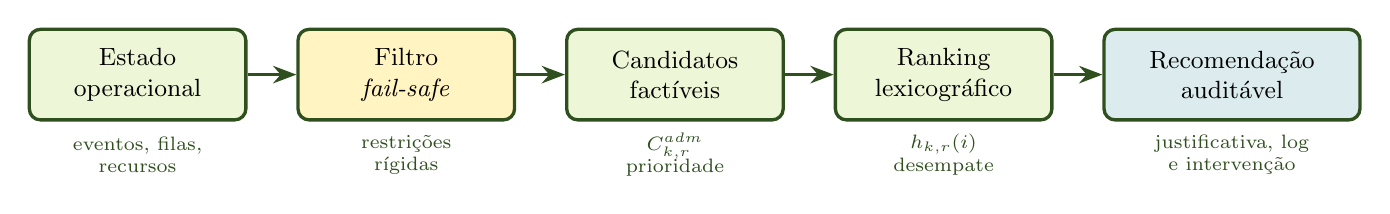
\begin{tikzpicture}[
  >=Stealth,
  font=\small,
  node distance=0.62cm,
  flowstep/.style={draw=pequiDark, very thick, rounded corners=4pt, align=center,
               minimum width=2.75cm, minimum height=1.15cm, fill=pequiLight},
  guard/.style={draw=pequiDark, very thick, rounded corners=4pt, align=center,
                minimum width=2.75cm, minimum height=1.15cm, fill=pequiPulpLight},
  final/.style={draw=pequiDark, very thick, rounded corners=4pt, align=center,
                minimum width=3.25cm, minimum height=1.15cm, fill=pequiBlue!55},
  flow/.style={->, very thick, draw=pequiDark}
]
\node[flowstep] (estado) {Estado\\operacional};
\node[guard, right=of estado] (filtro) {Filtro\\\textit{fail-safe}};
\node[flowstep, right=of filtro] (candidatos) {Candidatos\\fact\'iveis};
\node[flowstep, right=of candidatos] (ranking) {Ranking\\lexicogr\'afico};
\node[final, right=of ranking] (saida) {Recomenda\c{c}\~ao\\audit\'avel};

\draw[flow] (estado) -- (filtro);
\draw[flow] (filtro) -- (candidatos);
\draw[flow] (candidatos) -- (ranking);
\draw[flow] (ranking) -- (saida);

\node[font=\scriptsize, align=center, text=pequiDark] at ($(estado.south)+(0,-0.42)$)
  {eventos, filas,\\recursos};
\node[font=\scriptsize, align=center, text=pequiDark] at ($(filtro.south)+(0,-0.42)$)
  {restri\c{c}\~oes\\r\'igidas};
\node[font=\scriptsize, align=center, text=pequiDark] at ($(candidatos.south)+(0,-0.42)$)
  {$C^{adm}_{k,r}$\\prioridade};
\node[font=\scriptsize, align=center, text=pequiDark] at ($(ranking.south)+(0,-0.42)$)
  {$h_{k,r}(i)$\\desempate};
\node[font=\scriptsize, align=center, text=pequiDark] at ($(saida.south)+(0,-0.42)$)
  {justificativa, log\\e interven\c{c}\~ao};
\end{tikzpicture}%
}
\caption[Fluxo conceitual do artefato]{Fluxo conceitual do artefato principal proposto.}
\end{figure}

A Tabela~\ref{tab:taxonomia-restricoes-artefato} resume as classes de restri\c{c}\~ao que alimentam o filtro \textit{fail-safe} e o registro audit\'avel do artefato.

\begin{table}[H]
\centering
\small
\setlength{\tabcolsep}{6pt}
\renewcommand{\arraystretch}{1.16}
\begin{tabularx}{\textwidth}{@{}P{0.24\textwidth}P{0.32\textwidth}Y@{}}
\toprule
\rowcolor{tablehead}
\textbf{Classe} & \textbf{Crit\'erio operacional} & \textbf{Uso no artefato} \\
\midrule
Admissibilidade f\'isica & compatibilidade carga--recurso & remove candidatos incompat\'iveis antes do ranqueamento \\
\addlinespace
Admissibilidade administrativa & bloqueio documental ou sanit\'ario & impede despacho autom\'atico e exige justificativa \\
\addlinespace
Disponibilidade operacional & recurso bloqueado, em falha ou destino fechado por chuva & zera capacidade tempor\'aria e reabre decis\~ao apenas no retorno \\
\addlinespace
Preced\^encia mandat\'oria & prioridade operacional validada & antecede FIFO e crit\'erios de escore \\
\addlinespace
Governan\c{c}a humana & interven\c{c}\~ao autorizada e registrada & permite sobreposi\c{c}\~ao audit\'avel sem violar restri\c{c}\~oes r\'igidas \\
\bottomrule
\end{tabularx}
\caption[Taxonomia de restri\c{c}\~oes do artefato]{Taxonomia enxuta das restri\c{c}\~oes usadas pelo artefato. Os eventos que atualizam estado ficam consolidados na Tabela~\ref{tab:eventos-des}.}
\label{tab:taxonomia-restricoes-artefato}
\end{table}

\subsection{Arquitetura do modelo digital em Unreal Engine}

O modelo digital ser\'a implementado no \textbf{Unreal Engine~5.8} como camada de
apresenta\c{c}\~ao desacoplada da infer\^encia experimental. A cada execu\c{c}\~ao, o
simulador Python produzir\'a um fluxo versionado de estados e eventos com tempo simulado,
identificador do caminh\~ao, etapa, recurso, posi\c{c}\~ao l\'ogica, estado da fila,
perturba\c{c}\~ao e decis\~ao registrada. O Unreal importar\'a esse fluxo para animar o
leiaute e permitir pausa, avan\c{c}o e inspe\c{c}\~ao do replay. O c\'alculo de H1, A1 e A2
continuar\'a no ambiente experimental, a partir dos logs can\^onicos; o modelo digital n\~ao
recalcula m\'etricas nem altera resultados.

O projeto Unreal j\'a est\'a inicializado na vers\~ao~5.8, mas a cena de dom\'inio, os ativos,
o importador de eventos e os controles de replay ainda constituem trabalho do TCC~II. A
interface m\'inima entre simulador e modelo digital ser\'a JSONL com esquema versionado e
identifica\c{c}\~ao de cen\'ario, semente, pol\'itica e checksum dos par\^ametros. Essa
separa\c{c}\~ao permite validar os dados antes da visualiza\c{c}\~ao e evita acoplamento do
motor de despacho ao motor gr\'afico.

\section{Modelagem do despacho online}\label{ch:modelagem}
A modelagem delimita o problema como \textbf{despacho online por recurso liberado com horizonte curto}: a cada libera\c{c}\~ao de recurso, o artefato escolhe o pr\'oximo caminh\~ao fact\'ivel sob restri\c{c}\~oes operacionais. Sejam $T$ o conjunto de caminh\~oes, $R$ o conjunto de recursos operacionais, $E$ o conjunto de eventos disruptivos, $K$ o conjunto de instantes de decis\~ao e $O = \{1,2,3,4\}$ o conjunto ordenado de opera\c{c}\~oes do p\'atio: 1 = entrada, 2 = pesagem inicial, 3 = descarga e 4 = pesagem final. Cada recurso $r \in R$ atende um subconjunto de opera\c{c}\~oes $O(r) \subseteq O$, e cada caminh\~ao $i \in T$ possui hor\'ario de chegada, tipo de carga, prioridade, situa\c{c}\~ao documental e recursos eleg\'iveis por opera\c{c}\~ao.

A escolha f\'isica adotada nesta pesquisa \'e a de \textbf{balan\c{c}as compartilhadas}: o mesmo pool $B \subset R$ executa a pesagem bruta na etapa~2 e a tara na etapa~4, logo $O(r)=\{2,4\}$ para $r \in B$. Portaria e moegas permanecem recursos de etapa \'unica. Essa decis\~ao classifica o p\'atio como \textit{Dynamic Reentrant Hybrid Flow Shop} (RHFS): h\'a m\'ultiplas m\'aquinas paralelas por est\'agio, caracter\'istica do \textit{hybrid flow shop} \parencite{ruizHybridFlowShop2010, ribasReviewClassificationHybrid2010}, e h\'a reentr\^ancia porque caminh\~oes retornam ao mesmo tipo de instala\c{c}\~ao f\'isica, disputando as mesmas balan\c{c}as em dois pontos da rota \parencite{gravesSchedulingReentrantFlow1983}. Se as pesagens de entrada e sa\'ida fossem pools f\'isicos separados, o r\'otulo correto seria D-HFS; neste recorte, a conten\c{c}\~ao cruzada das balan\c{c}as torna a reentr\^ancia parte central do modelo.

O modelo computacional opera em quatro etapas sequenciais cr\'iticas: entrada no p\'atio, pesagem inicial, descarga e pesagem final. Essa fronteira isola gargalos, propaga\c{c}\~ao de atrasos, filas intermedi\'arias e bloqueio de recursos. O detalhamento segue Law: objetivos, medidas de desempenho, dados dispon\'iveis, valida\c{c}\~ao com especialistas/SMEs e sensibilidade governam o n\'ivel de detalhe; o modelo evita correspond\^encia um-para-um e excesso de granularidade \parencite[Sec.~5.2, p.~249--251]{lawSimulationModelingAnalysis2015}. A \'area de espera atua como buffer operacional entre etapas. As Figuras~\ref{fig:arquitetura-des}, \ref{fig:layout-patio} e \ref{fig:fluxo-operacional} mostram, respectivamente, a execu\c{c}\~ao DES, o leiaute esquem\'atico e o fluxo de um caminh\~ao.

\subsection{Arquitetura lógica da simulação de eventos discretos}

O simulador usa lista futura de eventos. O tempo simulado avan\c{c}a quando o pr\'oximo evento \'e processado e, quando aplic\'avel, agenda novos eventos. O executor DES chama o motor de despacho quando um recurso fica livre, um caminh\~ao se torna eleg\'ivel ou uma perturba\c{c}\~ao altera candidatos fact\'iveis.

\begin{figure}[H]
\centering
\resizebox{\textwidth}{!}{%
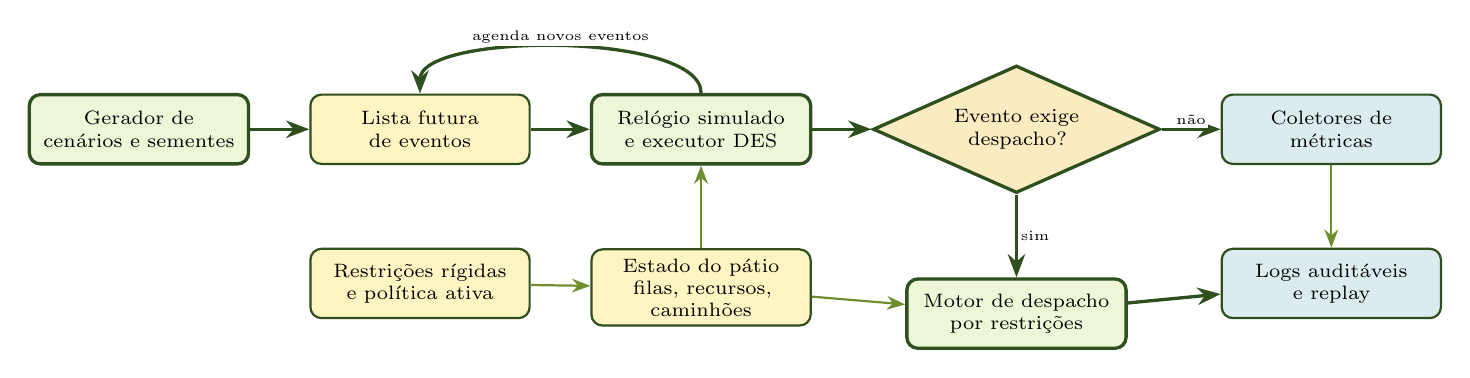
\begin{tikzpicture}[
  >=Stealth,
  font=\scriptsize,
  node distance=0.85cm and 0.75cm,
  process/.style={draw=pequiDark, very thick, rounded corners=4pt, align=center,
                  minimum height=0.88cm, text width=2.55cm, fill=pequiLight},
  store/.style={draw=pequiDark, thick, rounded corners=4pt, align=center,
                minimum height=0.88cm, text width=2.55cm, fill=pequiPulpLight},
  decision/.style={draw=pequiDark, very thick, diamond, aspect=2.25, align=center,
                   inner sep=1.2pt, text width=2.25cm, fill=pequiPulp!35},
  outputblock/.style={draw=pequiDark, thick, rounded corners=4pt, align=center,
                      minimum height=0.88cm, text width=2.55cm, fill=pequiBlue!55},
  line/.style={->, very thick, draw=pequiDark},
  softline/.style={->, thick, draw=pequiGreen}
]

\node[process] (scenario) {Gerador de\\cen\'arios e sementes};
\node[store, right=of scenario] (fel) {Lista futura\\de eventos};
\node[process, right=of fel] (clock) {Rel\'ogio simulado\\e executor DES};
\node[decision, right=of clock] (dispatch) {Evento exige\\despacho?};
\node[outputblock, right=of dispatch] (metrics) {Coletores de\\m\'etricas};

\node[store, below=1.05cm of fel] (rules) {Restri\c{c}\~oes r\'igidas\\e pol\'itica ativa};
\node[store, below=1.05cm of clock] (state) {Estado do p\'atio\\filas, recursos, caminh\~oes};
\node[process, below=1.05cm of dispatch] (engine) {Motor de despacho\\por restri\c{c}\~oes};
\node[outputblock, below=1.05cm of metrics] (logs) {Logs audit\'aveis\\e replay};

\draw[line] (scenario) -- (fel);
\draw[line] (fel) -- (clock);
\draw[line] (clock) -- (dispatch);
\draw[line] (dispatch) -- node[above, font=\tiny, fill=white, inner sep=1pt]{n\~ao} (metrics);
\draw[line] (dispatch) -- node[right, font=\tiny, fill=white, inner sep=1pt]{sim} (engine);
\draw[line] (engine) -- (logs);
\draw[softline] (rules) -- (state);
\draw[softline] (state) -- (engine);
\draw[softline] (state) -- (clock);
\draw[softline] (metrics) -- (logs);
\draw[line] (clock.north) .. controls +(0,0.78) and +(0,0.78) ..
  node[above, font=\tiny, fill=white, inner sep=1pt]{agenda novos eventos} (fel.north);

\end{tikzpicture}%
}
\caption[Arquitetura l\'ogica do simulador]{Arquitetura l\'ogica do simulador de eventos discretos usado para avaliar as pol\'iticas de despacho.}
\label{fig:arquitetura-des}
\end{figure}

Cada cen\'ario define chegadas, recursos, tempos de processamento, eventos disruptivos e semente. O estado do p\'atio armazena posi\c{c}\~ao dos caminh\~oes, filas por etapa, disponibilidade dos recursos, bloqueios, chuva e prioridades. Quando um evento exige decis\~ao, o executor consulta a pol\'itica ativa: FIFO estrito, FIFO \textit{flow-faithful}, prioridade + factibilidade local, escore fixo ou artefato proposto. A decis\~ao agenda atendimento, atualiza filas e recursos e emite logs para auditoria e m\'etricas.

\begin{table}[H]
\centering
\small
\setlength{\tabcolsep}{5pt}
\renewcommand{\arraystretch}{1.18}
\begin{tabularx}{\textwidth}{@{}P{0.22\textwidth}P{0.33\textwidth}Y@{}}
\toprule
\rowcolor{tablehead}
\textbf{Evento DES} & \textbf{Atualiza\c{c}\~ao de estado} & \textbf{Eventos ou registros gerados} \\
\midrule
Chegada ao p\'atio & cria caminh\~ao, registra atributos, insere na fila da etapa 1 & tentativa de despacho se houver portaria livre \\
\addlinespace
Fim de atendimento em uma etapa & libera recurso, move caminh\~ao para buffer da pr\'oxima etapa ou finaliza o ciclo & novo evento de recurso livre e, se houver pr\'oxima etapa, tentativa de despacho \\
\addlinespace
Recurso livre & consulta fila e conjunto de candidatos eleg\'iveis para o recurso & chamada da pol\'itica de despacho; agenda in\'icio/fim de atendimento quando h\'a candidato fact\'ivel \\
\addlinespace
Bloqueio ou libera\c{c}\~ao documental & altera elegibilidade do caminh\~ao afetado & registro de bloqueio/libera\c{c}\~ao e reavalia\c{c}\~ao de candidatos na etapa corrente \\
\addlinespace
In\'icio ou fim de chuva & altera disponibilidade de destinos abertos sens\'iveis & reavalia\c{c}\~ao dos recursos afetados e registro da causa ambiental \\
\addlinespace
Falha ou retorno de recurso & altera capacidade do recurso e, se necess\'ario, interrompe novas aloca\c{c}\~oes & registro de indisponibilidade; reprograma\c{c}\~ao de candidatos ainda n\~ao atendidos \\
\addlinespace
Interven\c{c}\~ao humana & tenta substituir ou confirmar a recomenda\c{c}\~ao do sistema & aceita se respeitar restri\c{c}\~oes r\'igidas; caso contr\'ario, registra bloqueio da interven\c{c}\~ao \\
\bottomrule
\end{tabularx}
\caption[Eventos do simulador DES]{Tipos de evento processados pelo simulador DES e suas consequ\^encias operacionais.}
\label{tab:eventos-des}
\end{table}

A arquitetura separa responsabilidades: o \textbf{simulador} controla tempo, eventos, filas, recursos e amostragem; a \textbf{pol\'itica de despacho} escolhe o pr\'oximo caminh\~ao fact\'ivel; e os \textbf{coletores} geram m\'etricas e logs. Todas as pol\'iticas observam o mesmo estado, sob a mesma semente, e diferem pela regra de sele\c{c}\~ao.

% ----------------------------------------------------------------
% Figura 1: Leiaute esquem\'atico do p\'atio (vista superior)
% ----------------------------------------------------------------
\begin{figure}[H]
\centering
\resizebox{\textwidth}{!}{%
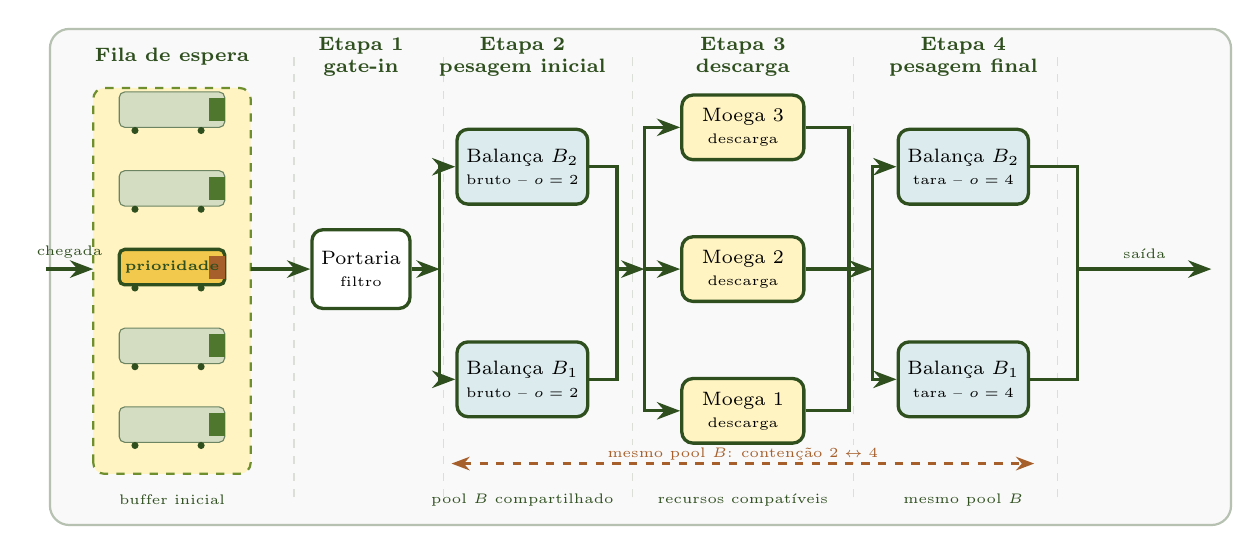
\begin{tikzpicture}[
  >=Stealth,
  font=\scriptsize,
  flow/.style={->, very thick, draw=pequiDark},
  connector/.style={very thick, draw=pequiDark},
  cross/.style={<->, thick, dashed, draw=pequiEarth},
  stagebox/.style={draw=pequiDark, very thick, rounded corners=4pt, align=center},
  label/.style={font=\scriptsize\bfseries, text=pequiDark, align=center}
]

  \fill[gray!5, rounded corners=7pt] (0,0) rectangle (15,6.3);
  \draw[pequiDark!35, thick, rounded corners=7pt] (0,0) rectangle (15,6.3);

  \foreach \x in {3.1,5.0,7.4,10.2,12.8} {
    \draw[pequiDark!18, dashed] (\x,0.35) -- (\x,5.95);
  }

  \node[label] at (1.55,5.95) {Fila de espera};
  \node[label] at (3.95,5.95) {Etapa 1\\gate-in};
  \node[label] at (6.0,5.95) {Etapa 2\\pesagem inicial};
  \node[label] at (8.8,5.95) {Etapa 3\\descarga};
  \node[label] at (11.6,5.95) {Etapa 4\\pesagem final};

  \fill[pequiPulpLight, rounded corners=4pt] (0.55,0.65) rectangle (2.55,5.55);
  \draw[pequiGreen, thick, dashed, rounded corners=4pt] (0.55,0.65) rectangle (2.55,5.55);

  \foreach \y in {1.05,2.05,4.05,5.05} {
    \filldraw[fill=pequiGreen!30, draw=pequiDark!70, rounded corners=2pt] (0.88,\y) rectangle (2.22,\y+0.45);
    \fill[pequiLeaf] (2.02,\y+0.08) rectangle (2.22,\y+0.37);
    \fill[pequiDark] (1.08,\y-0.04) circle (0.045);
    \fill[pequiDark] (1.92,\y-0.04) circle (0.045);
  }
  \filldraw[fill=pequiPulp, draw=pequiDark, very thick, rounded corners=2pt] (0.88,3.05) rectangle (2.22,3.50);
  \fill[pequiEarth] (2.02,3.13) rectangle (2.22,3.42);
  \fill[pequiDark] (1.08,3.01) circle (0.045);
  \fill[pequiDark] (1.92,3.01) circle (0.045);
  \node[font=\tiny\bfseries, text=pequiDark] at (1.55,3.28) {prioridade};

  \node[stagebox, fill=white, minimum width=1.05cm, minimum height=1.0cm] (gate) at (3.95,3.25)
    {Portaria\\{\tiny filtro}};

  \node[stagebox, fill=pequiBlue!55, minimum width=1.45cm, minimum height=0.95cm] (scaleA) at (6.0,4.55)
    {Balan\c{c}a $B_2$\\{\tiny bruto -- $o=2$}};
  \node[stagebox, fill=pequiBlue!55, minimum width=1.45cm, minimum height=0.95cm] (scaleB) at (6.0,1.85)
    {Balan\c{c}a $B_1$\\{\tiny bruto -- $o=2$}};

  \node[stagebox, fill=pequiPulpLight, minimum width=1.55cm, minimum height=0.82cm] (hopperA) at (8.8,5.05)
    {Moega 3\\{\tiny descarga}};
  \node[stagebox, fill=pequiPulpLight, minimum width=1.55cm, minimum height=0.82cm] (hopperB) at (8.8,3.25)
    {Moega 2\\{\tiny descarga}};
  \node[stagebox, fill=pequiPulpLight, minimum width=1.55cm, minimum height=0.82cm] (hopperC) at (8.8,1.45)
    {Moega 1\\{\tiny descarga}};

  \node[stagebox, fill=pequiBlue!55, minimum width=1.45cm, minimum height=0.95cm] (scaleOutA) at (11.6,4.55)
    {Balan\c{c}a $B_2$\\{\tiny tara -- $o=4$}};
  \node[stagebox, fill=pequiBlue!55, minimum width=1.45cm, minimum height=0.95cm] (scaleOutB) at (11.6,1.85)
    {Balan\c{c}a $B_1$\\{\tiny tara -- $o=4$}};

  \draw[flow] (-0.05,3.25) -- (0.55,3.25) node[midway, above, font=\tiny, text=pequiDark]{chegada};
  \draw[flow] (2.55,3.25) -- (gate.west);
  \coordinate (afterGate) at (4.95,3.25);
  \coordinate (afterScales) at (7.20,3.25);
  \coordinate (afterHoppers) at (10.15,3.25);
  \coordinate (beforeOutScales) at (10.45,3.25);
  \coordinate (afterOutScales) at (13.05,3.25);

  \draw[flow] (gate.east) -- (afterGate);
  \draw[flow] (afterGate) |- (scaleA.west);
  \draw[flow] (afterGate) |- (scaleB.west);

  \draw[connector] (scaleA.east) -| (afterScales);
  \draw[connector] (scaleB.east) -| (afterScales);
  \draw[flow] (afterScales) -- (7.55,3.25);
  \draw[flow] (7.55,3.25) |- (hopperA.west);
  \draw[flow] (7.55,3.25) -- (hopperB.west);
  \draw[flow] (7.55,3.25) |- (hopperC.west);

  \draw[connector] (hopperA.east) -| (afterHoppers);
  \draw[connector] (hopperB.east) -- (afterHoppers);
  \draw[connector] (hopperC.east) -| (afterHoppers);
  \draw[flow] (afterHoppers) -- (beforeOutScales);
  \draw[flow] (beforeOutScales) |- (scaleOutA.west);
  \draw[flow] (beforeOutScales) |- (scaleOutB.west);

  \draw[connector] (scaleOutA.east) -| (afterOutScales);
  \draw[connector] (scaleOutB.east) -| (afterOutScales);
  \draw[flow] (afterOutScales) -- (14.75,3.25) node[midway, above, font=\tiny, text=pequiDark]{sa\'ida};

  \draw[cross] (5.10,0.78) -- node[above, font=\tiny, text=pequiEarth, fill=gray!5, inner sep=1pt]
    {mesmo pool $B$: conten\c{c}\~ao $2 \leftrightarrow 4$} (12.50,0.78);

  \node[font=\tiny, text=pequiDark] at (1.55,0.32) {buffer inicial};
  \node[font=\tiny, text=pequiDark] at (6.0,0.32) {pool $B$ compartilhado};
  \node[font=\tiny, text=pequiDark] at (8.8,0.32) {recursos compat\'iveis};
  \node[font=\tiny, text=pequiDark] at (11.6,0.32) {mesmo pool $B$};

\end{tikzpicture}%
}
\caption[Leiaute esquem\'atico do p\'atio]{Leiaute esquem\'atico do p\'atio de recebimento de gr\~aos (vista superior), com quatro etapas operacionais e balan\c{c}as f\'isicas compartilhadas. \textbf{Etapa~1}: gate-in (portaria). \textbf{Etapa~2}: peso bruto no pool $B$ de balan\c{c}as. \textbf{Etapa~3}: descarga (moegas). \textbf{Etapa~4}: tara no mesmo pool $B$. As setas tracejadas indicam a conten\c{c}\~ao reentrante entre as etapas~2 e~4; caminh\~oes com prioridade mandat\'oria est\~ao destacados em amarelo-pequi.}
\label{fig:layout-patio}
\end{figure}

% ----------------------------------------------------------------
% Figura 2: Fluxo operacional nas quatro etapas
% ----------------------------------------------------------------
\begin{figure}[H]
\centering
\resizebox{\textwidth}{!}{%
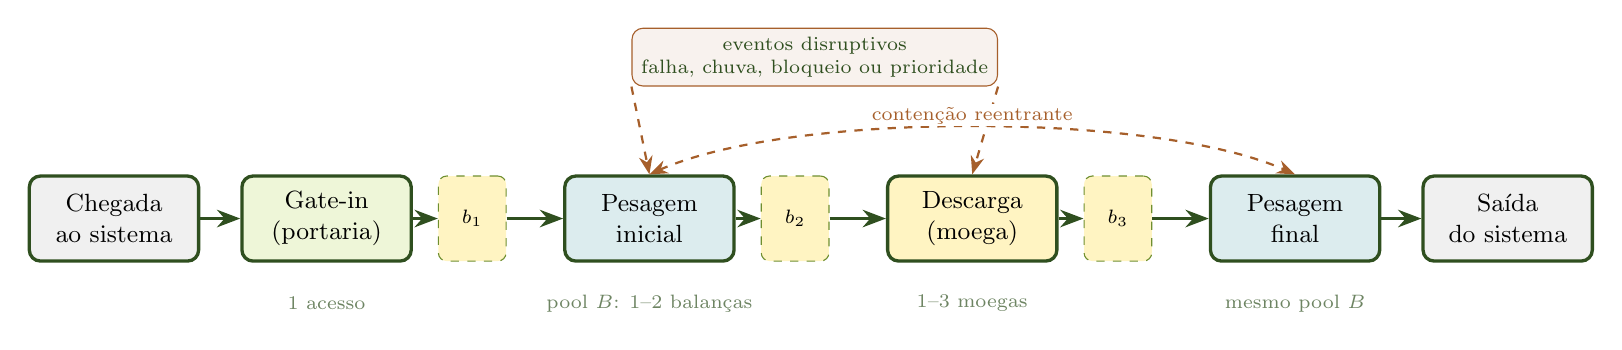
\begin{tikzpicture}[>=Stealth, font=\small,
    flowstep/.style={draw=pequiDark, very thick, rounded corners=4pt, minimum width=2.15cm,
                     minimum height=1.08cm, align=center},
    buf/.style={draw=pequiGreen, rounded corners=3pt, minimum width=0.86cm,
                minimum height=1.08cm, align=center, fill=pequiPulpLight,
                dashed, font=\scriptsize},
    lbl/.style={font=\scriptsize, text=pequiDark!70, align=center},
    flow/.style={->, very thick, draw=pequiDark},
    event/.style={->, dashed, thick, draw=pequiEarth},
    shared/.style={<->, dashed, thick, draw=pequiEarth}]

  \node[flowstep, fill=gray!12]       (arr) at (0,0)    {Chegada\\ao sistema};
  \node[flowstep, fill=pequiLight]    (g1)  at (2.7,0)  {Gate-in\\(portaria)};
  \node[buf]                     (b1)  at (4.55,0) {$b_1$};
  \node[flowstep, fill=pequiBlue!55]  (w1)  at (6.8,0)  {Pesagem\\inicial};
  \node[buf]                     (b2)  at (8.65,0) {$b_2$};
  \node[flowstep, fill=pequiPulpLight](dsc) at (10.9,0) {Descarga\\(moega)};
  \node[buf]                     (b3)  at (12.75,0) {$b_3$};
  \node[flowstep, fill=pequiBlue!55]  (w2)  at (15.0,0) {Pesagem\\final};
  \node[flowstep, fill=gray!12]       (out) at (17.7,0) {Sa\'ida\\do sistema};

  \foreach \a/\b in {arr/g1,g1/b1,b1/w1,w1/b2,b2/dsc,dsc/b3,b3/w2,w2/out} {
    \draw[flow] (\a) -- (\b);
  }

  \node[lbl] at (2.7,-1.08)  {1 acesso};
  \node[lbl] at (6.8,-1.08)  {pool $B$: 1--2 balan\c{c}as};
  \node[lbl] at (10.9,-1.08) {1--3 moegas};
  \node[lbl] at (15.0,-1.08) {mesmo pool $B$};

  \node[draw=pequiEarth, fill=pequiEarth!8, rounded corners=4pt,
        font=\scriptsize, text=pequiDark, align=center, minimum width=4.25cm] (ev) at (8.9,2.05)
        {eventos disruptivos\\falha, chuva, bloqueio ou prioridade};
  \draw[event] (ev.south west) -- (w1.north);
  \draw[event] (ev.south east) -- (dsc.north);
  \draw[shared] (w1.north) .. controls (8.6,1.36) and (13.2,1.36) ..
    node[above, font=\scriptsize, text=pequiEarth, fill=white, inner sep=1pt]{conten\c{c}\~ao reentrante}
    (w2.north);

\end{tikzpicture}%
}% end resizebox
\caption[Fluxo operacional do caminh\~ao]{Fluxo operacional de um caminh\~ao pelas quatro etapas do modelo de p\'atio. Buffers intermedi\'arios ($b_k$) acomodam filas entre etapas. A pesagem inicial e a pesagem final usam o mesmo pool f\'isico de balan\c{c}as; por isso, a libera\c{c}\~ao de uma balan\c{c}a pode escolher caminh\~ao de tara ou de peso bruto. As setas tracejadas indicam classes de eventos disruptivos e a conten\c{c}\~ao reentrante entre as etapas~2 e~4.}
\label{fig:fluxo-operacional}
\end{figure}

\subsection{Formula\c{c}\~ao matem\'atica do despacho online}
\label{sec:formulacao-despacho}

A formula\c{c}\~ao distingue restri\c{c}\~oes r\'igidas, estado do sistema e regra local de sele\c{c}\~ao. O problema global de escalonamento do p\'atio --- minimizar \textit{makespan} ou espera agregada respeitando preced\^encias, capacidade e restri\c{c}\~oes r\'igidas --- \'e um problema de otimiza\c{c}\~ao combinat\'oria de dif\'icil tratabilidade sob escala e dinamismo; o Ap\^endice~\ref{apx:materiais-contextuais} reporta, no artefato congelado, que inst\^ancias m\'edias sob regime \textit{disrupted} n\~ao atingem \'otimo de \textit{makespan} em or\c{c}amento de 60~s com \textit{solver} exato, acumulando \textit{gaps} de at\'e 14{,}4\%. Esse perfil de intratabilidade motiva, em vez da otimiza\c{c}\~ao global a cada evento, uma heur\'istica construtiva \textit{online} (regra de despacho) que decide localmente por recurso liberado, coerente com o uso de l\'ogicas locais sobre simula\c{c}\~ao de eventos discretos em ambientes din\^amicos e incertos \parencite{torbaliMultiagentbasedRealtimeTruck2023,fonsecaStabilityApproachCDC2025}.

No instante~$k$, o estado do sistema \'e representado por
\[
S_k = \langle \pi_k, u_k, b_k, d_k, m_k \rangle,
\]
em que $\pi_k$ \'e a fila ativa por opera\c{c}\~ao, $u_k$ registra a pr\'oxima disponibilidade de cada recurso f\'isico, $b_k$ a ocupa\c{c}\~ao do \textit{buffer}, $d_k$ agrega atributos de documentos/prioridade e $m_k$ representa o modo operacional do p\'atio, incluindo chuva e indisponibilidades. Seja $q_i(k) \in O$ a pr\'oxima opera\c{c}\~ao pendente do caminh\~ao~$i$. Quando um recurso~$r$ \'e liberado no instante~$k$, a decis\~ao incide sobre esse recurso e sobre todas as filas de opera\c{c}\~oes atendidas por~$r$:
\[
C_{k,r} = \bigcup_{o \in O(r)} C^{(o)}_{k,r},
\qquad
C^{(o)}_{k,r} =
\{\,i \in \pi_{k,o}: q_i(k)=o,\; r \in R_i(o),\; \mathcal{F}_{i,r}(k)=1\,\}.
\]
Assim, para uma balan\c{c}a f\'isica $r \in B$, tem-se $C_{k,r}=C^{(2)}_{k,r}\cup C^{(4)}_{k,r}$: caminh\~oes aguardando peso bruto e caminh\~oes aguardando tara competem pelo mesmo evento de recurso livre. O mesmo registro $u_{k,r}$ controla a pr\'oxima disponibilidade da balan\c{c}a em ambas as opera\c{c}\~oes; n\~ao existem calend\'arios independentes para entrada e sa\'ida. O indicador $\mathcal{F}_{i,r}(k)$ vale 1 somente quando todas as restri\c{c}\~oes r\'igidas s\~ao satisfeitas. Em termos de factibilidade, $C^{(o)}_{k,r}$ re\'une os caminh\~oes~$i$ tais que: (i)~$i$ j\'a chegou ao sistema; (ii)~a opera\c{c}\~ao anterior de~$i$ est\'a conclu\'ida; (iii)~$r$ pertence ao conjunto de recursos eleg\'iveis para $q_i(k)$; (iv)~$\mathrm{cap}_r(k) > 0$; (v)~$\mathrm{comp}_{i,r} = 1$; (vi)~$\mathrm{doc}_i(k) = 1$; (vii)~$\mathrm{clima}_{i,r}(k) = 1$; e (viii)~$b_k$ ainda comporta a transi\c{c}\~ao para a pr\'oxima fila, quando houver pr\'oxima fila. Inviabilidade n\~ao entra como penalidade branda: candidatos invi\'aveis s\~ao removidos antes de qualquer ranqueamento. Quando $C_{k,r} = \emptyset$, o motor n\~ao emite despacho para aquele recurso; registra a impossibilidade e a regra bloqueadora correspondente.

A prioridade operacional \'e codificada por $p(i) \in \{0, 1, 2\}$, em que~$2$ denota prioridade mandat\'oria, e o subconjunto $C^{2}_{k,r} = \{ i \in C_{k,r} : p(i) = 2 \}$ re\'une os candidatos mandat\'orios.

A janela curta $H_0 = 6$ n\~ao \'e aplicada como truncagem cega de urg\^encia. Antes do ranqueamento, o motor forma o \emph{dom\'inio admiss\'ivel} $C^{adm}_{k,r}$ segundo duas regras determin\'isticas, hierarquizadas. Se houver candidato com prioridade mandat\'oria, o dom\'inio \'e reduzido a~$C^{2}_{k,r}$ \emph{na \'integra}, independentemente de~$H_0$, pois a prioridade mandat\'oria antecede a janela curta e qualquer crit\'erio de estabilidade. Na aus\^encia de prioridade mandat\'oria, o dom\'inio combina os $H_0$ primeiros candidatos fact\'iveis por ordem de chegada \`a opera\c{c}\~ao corrente com \emph{todos} os candidatos fact\'iveis que j\'a violaram seu limiar operacional de espera, isto \'e, com press\~ao operacional positiva:

\begin{equation}
C^{adm}_{k,r} =
\begin{cases}
  C^{2}_{k,r}, & \text{se } C^{2}_{k,r} \neq \emptyset; \\[2pt]
  \mathrm{Top}^{\,\text{chegada}}_{H_0}(C_{k,r}) \;\cup\;
  \{\, i \in C_{k,r} : \mathrm{pressure}_i(k) > 0 \,\}, & \text{caso contr\'ario.}
\end{cases}
\label{eq:cadm}
\end{equation}

\noindent em que $\mathrm{pressure}_i(k) = \max\{0, -\mathrm{slack}_i(k)\}$ e $\mathrm{slack}_i(k) = \tau_{p(i)} - W_i(k)$. Assim, $H_0$ limita apenas a competi\c{c}\~ao \emph{ordin\'aria} e a profundidade de reordena\c{c}\~ao entre candidatos n\~ao cr\'iticos, enquanto os limiares~$\tau_p$ determinam a entrada de candidatos \emph{cr\'iticos} no dom\'inio de decis\~ao. A janela governa o ordin\'ario; o limiar governa a urg\^encia.

Em termos operacionais, o motor considera caminh\~oes aptos para a opera\c{c}\~ao corrente, compat\'iveis com o recurso dispon\'ivel e livres de bloqueios documentais, clim\'aticos ou operacionais. No caso das balan\c{c}as, essa opera\c{c}\~ao corrente pode ser~2 ou~4 no mesmo conjunto de candidatos, o que explicita a conten\c{c}\~ao cruzada da reentr\^ancia.

A decis\~ao do motor no evento $(k,r)$ \'e a sele\c{c}\~ao do candidato que maximiza o vetor de atributos em ordem lexicogr\'afica, ou a ociosidade for\c{c}ada quando n\~ao h\'a op\c{c}\~ao segura:

\begin{equation}
y_{k,r} =
\begin{cases}
  \displaystyle \operatorname*{arg\,lexmax}_{\,i \in C^{adm}_{k,r}}\;
  h_{k,r}(i), & \text{se } C^{adm}_{k,r} \neq \emptyset; \\[6pt]
  \emptyset, & \text{caso contr\'ario (ociosidade/bloqueio registrado).}
\end{cases}
\label{eq:selecao}
\end{equation}

\noindent com o vetor de avalia\c{c}\~ao
\[
  h_{k,r}(i) = \big\langle\, \hat{P}_i(k),\; \hat{W}_i(k),\;
  -\hat{R}_{k,r}(i),\; \hat{A}_{i,r}(k) \,\big\rangle,
\]
em que $\hat{P}_i(k)$ \'e a press\~ao operacional normalizada, $\hat{W}_i(k)$ a espera normalizada na opera\c{c}\~ao corrente~$q_i(k)$, $\hat{R}_{k,r}(i)$ a penalidade normalizada de reordena\c{c}\~ao e $\hat{A}_{i,r}(k)$ a afinidade imediata de \emph{setup}. O termo $W_i(k)$ denota o tempo aguardado desde a elegibilidade para a opera\c{c}\~ao corrente. As normaliza\c{c}\~oes s\~ao calculadas \emph{dentro} de~$C^{adm}_{k,r}$:
\[
  \hat{P}_i(k) = \frac{\mathrm{pressure}_i(k)}
  {\max_{j \in C^{adm}_{k,r}} \mathrm{pressure}_j(k)}, \qquad
  \hat{W}_i(k) = \frac{W_i(k)}{\max_{j \in C^{adm}_{k,r}} W_j(k)},
\]
quando os denominadores forem positivos; denominadores nulos produzem componente igual a~$0$. A penalidade de reordena\c{c}\~ao \'e dada por
\[
\hat{R}_{k,r}(i)=\frac{R_{k,r}(i)}{\max(1, |C^{adm}_{k,r}|-1)}.
\]
Se $y_{k,r}=i$, a transi\c{c}\~ao de estado registra $s_{i,q_i(k)} = k$, $c_{i,q_i(k)} = k + p^{(k)}_{i,q_i(k),r}$ e $u^{k+1}_r = c_{i,q_i(k)}$, preservando preced\^encia entre etapas e capacidade do \emph{buffer}. Para $r \in B$, essa atualiza\c{c}\~ao bloqueia a mesma balan\c{c}a tanto para candidatos de peso bruto quanto para novos candidatos de tara at\'e $u^{k+1}_r$. A afinidade $\hat{A}_{i,r}(k)$ vale 1 quando o recurso j\'a est\'a pronto para a classe de carga sem limpeza/setup; vale 0 quando existe setup admiss\'ivel. Compatibilidade carga--recurso entra como restri\c{c}\~ao r\'igida antes da afinidade.

O ordenamento lexicogr\'afico representa a assimetria operacional do dom\'inio de gr\~aos. No escoamento de safra, compromissos de atendimento t\^em natureza hier\'arquica e n\~ao compensat\'oria: um ganho na espera~$\hat{W}$ de um candidato n\~ao pode preterir a urg\^encia operacional~$\hat{P}$ de outro. Por constru\c{c}\~ao, qualquer diferen\c{c}a em~$\hat{P}_i(k)$ prevalece sobre diferen\c{c}as em~$\hat{W}_i(k)$. Diferentemente de uma soma ponderada escalar, o operador $\operatorname{arg\,lexmax}$ imp\~oe obedi\^encia estrita \`a hierarquia dos crit\'erios. Caso se deseje resolver a mesma regra em um solucionador alg\'ebrico, a forma lexicogr\'afica admite reescrita equivalente como soma escalar com coeficientes hier\'arquicos $M_1 \gg M_2 \gg M_3 \gg M_4 > 0$, sem que ganho em componente inferior compense perda em componente superior; essa equival\^encia \'e apenas notacional e n\~ao \'e o mecanismo implementado.

A sele\c{c}\~ao~\eqref{eq:selecao} \'e resolvida por varredura linear com comparador lexicogr\'afico, em custo $O(|C^{adm}_{k,r}|)$ por evento, sem necessidade de \emph{solver} de Programa\c{c}\~ao Inteira. Em aus\^encia de prioridade mandat\'oria, $|C^{adm}_{k,r}|$ pode crescer nos estratos de alta congest\~ao \`a medida que mais candidatos acumulam press\~ao positiva simult\^anea; esse crescimento n\~ao \'e ru\'ido, mas o pr\'oprio sinal que H1 busca, pois corresponde aos caminh\~oes cujo ranqueamento por urg\^encia o motor deve preservar. A expans\~ao cr\'itica n\~ao dilui a localidade da decis\~ao: ela apenas garante que o vencedor segundo o crit\'erio dominante nunca seja descartado pela ordem de chegada. O ranking exclui ociosidade do recurso porque, em $(k,r)$, esse termo \'e constante para todos os candidatos. Justificativa leg\'ivel, falha segura e interven\c{c}\~ao humana ficam auditadas em log.

Operacionalmente, o motor atualiza $S_k$ com chegadas, libera\c{c}\~oes, falhas, recupera\c{c}\~oes e mudan\c{c}as de prioridade. Em eventos simult\^aneos, processa primeiro libera\c{c}\~oes, depois falhas ou recupera\c{c}\~oes, mudan\c{c}as de prioridade e, por fim, chegadas; a decis\~ao de despacho ocorre depois dessa atualiza\c{c}\~ao. Para cada recurso livre $r$, o motor constr\'oi $C_{k,r}$ a partir da uni\~ao das filas em $O(r)$, registra bloqueio se o conjunto estiver vazio, ou forma $C^{adm}_{k,r}$ pela Equa\c{c}\~ao~\eqref{eq:cadm} e seleciona $y_{k,r}$ pela Equa\c{c}\~ao~\eqref{eq:selecao}. Empates usam prioridade, chegada \`a opera\c{c}\~ao corrente e identificador. Com m\'ultiplos recursos livres, a chave congelada ``menor opera\c{c}\~ao atendida, classe do recurso, identificador'' define a ordem; isso mant\'em determinismo sem duplicar a balan\c{c}a compartilhada em duas filas de recurso. Cada aloca\c{c}\~ao atualiza $S_k$ e registra recomenda\c{c}\~ao, justificativa e eventual interven\c{c}\~ao humana.

No painel confirmat\'orio de H1, a forma\c{c}\~ao de $C^{adm}_{k,r}$ --- filtro de factibilidade, redu\c{c}\~ao por prioridade mandat\'oria e expans\~ao por press\~ao positiva --- pertence \`a plataforma experimental compartilhada: todas as pol\'iticas comparadas observam o mesmo dom\'inio admiss\'ivel, sob a mesma semente e o mesmo estado. Varia exclusivamente a regra de sele\c{c}\~ao sobre $C^{adm}_{k,r}$. Assim, eventuais ganhos do artefato em~H1 s\~ao atribu\'iveis ao ranqueamento lexicogr\'afico, e n\~ao a uma regra de admiss\~ao privativa do motor.

\subsection{Pseudocódigo do motor de despacho}
O pseudoc\'odigo da Figura~\ref{fig:motor-despacho} traduz a modelagem em fluxo execut\'avel, com ordem determin\'istica dos eventos, forma\c{c}\~ao de candidatos, restri\c{c}\~oes r\'igidas, dom\'inio admiss\'ivel, desempate e registro audit\'avel.

\begin{figure}[H]
\centering
{\scriptsize
\noindent{\color{pequiDark}\rule{0.94\textwidth}{0.8pt}}\par\vspace{2pt}
\begin{minipage}{0.94\textwidth}
\begin{verbatim}
Motor de despacho online do artefato proposto
Entrada:
  S_k: estado operacional no instante k
  E_k: eventos observados no instante k
  R: recursos operacionais
  H0: tamanho da janela ordinaria local, fixado em 6
Saida:
  D_k: decisoes de despacho, bloqueios e registros auditaveis

1. ordenar E_k por: liberacoes -> falhas/recuperacoes -> prioridades -> chegadas
2. para cada evento e em E_k:
3.     atualizar S_k com chegadas, liberacoes, falhas, chuva ou prioridades
4. fim
5. D_k <- conjunto vazio
6. R_livre <- recursos fisicos livres em k, ordenados por menor operacao,
      classe e identificador
7. para cada recurso r em R_livre:
8.     F <- uniao das filas das operacoes em O(r)
       (para balanca compartilhada: etapas 2 e 4)
9.     C <- conjunto vazio
10.    para cada caminhao i em F:
11.        se i chegou, a operacao anterior de q_i(k) terminou
           e r atende q_i(k) entao
12.            se capacidade, compatibilidade, documento, clima e buffer
13.               forem todos validos entao
14.                adicionar i a C
15.            senao
16.                registrar regra bloqueadora de i para r
17.            fim
18.        fim
19.    fim
20.    se C estiver vazio entao
21.        registrar bloqueio: sem candidato factivel para r
22.        adicionar bloqueio a D_k
23.        continuar para o proximo recurso
24.    fim
25.    se existir candidato em C com prioridade mandataria entao
26.        C_adm <- todos os candidatos de C com prioridade mandataria
27.    senao
28.        C_fifo <- primeiros H0 candidatos de C na ordem de chegada a operacao
           corrente
29.        C_crit <- candidatos i de C com pressao operacional positiva
30.        C_adm <- uniao(C_fifo, C_crit)
31.    fim
32.    para cada candidato i em C_adm:
33.        calcular pressao normalizada P_i(k), espera normalizada W_i(k),
34.            penalidade de reordenacao R_i(k,r) e afinidade A_i(k,r)
35.        h_i <- <P_i(k), W_i(k), -R_i(k,r), A_i(k,r)>
36.    fim
37.    y <- candidato de C_adm com maior h_i em ordem lexicografica
38.    se houver empate entao
39.        desempatar por prioridade, chegada a operacao corrente e identificador
40.    fim
41.    gerar justificativa com candidato, recurso, regras e quebra de FIFO
42.    se houver intervencao humana autorizada entao
43.        validar que a intervencao nao viola restricoes rigidas
44.        registrar motivo textual da intervencao
45.        se a intervencao for factivel entao y <- escolha do operador
46.    fim
47.    despachar y para r, atualizar u_r e atualizar S_k
48.    adicionar decisao e registro correspondente a D_k
49. fim
50. retornar D_k
\end{verbatim}
\end{minipage}
\par\vspace{2pt}{\color{pequiDark}\rule{0.94\textwidth}{0.8pt}}
}
\caption[Pseudoc\'odigo do motor de despacho]{Pseudoc\'odigo do motor de despacho online proposto.}
\label{fig:motor-despacho}
\end{figure}
\section{Configuração do Simulador e Cenários}
O arcabou\c{c}o metodol\'ogico adotado \'e o Design Science Research, por ser o mais coerente com a constru\c{c}\~ao e avalia\c{c}\~ao de um artefato computacional voltado a um problema log\'istico complexo \parencite{hevnerDesignScienceInformation2004a, peffersDesignScienceResearch2007aa}. O artefato principal deste trabalho \'e o \textbf{motor de decis\~ao orientado a eventos}; o \textbf{simulador de eventos discretos} estabelece o ambiente de demonstra\c{c}\~ao e avalia\c{c}\~ao do artefato. O processo de pesquisa ser\'a estruturado nas seguintes fases:
\begin{enumerate}[leftmargin=1.27cm,itemsep=0pt,topsep=0pt,parsep=0pt,partopsep=0pt]
  \item Identifica\c{c}\~ao e delimita\c{c}\~ao do problema a partir do contexto operacional estudado;
  \item Elicita\c{c}\~ao dos requisitos funcionais e restri\c{c}\~oes do artefato, incluindo regras de neg\'ocio, restri\c{c}\~oes r\'igidas e crit\'erios de prioriza\c{c}\~ao;
  \item Modelagem formal do problema e defini\c{c}\~ao da estrat\'egia de decis\~ao;
  \item Desenvolvimento de um prot\'otipo com pol\'iticas de refer\^encia comparativas para avalia\c{c}\~ao;
  \item Demonstra\c{c}\~ao e avalia\c{c}\~ao do prot\'otipo em cen\'arios simulados;
  \item Discuss\~ao dos resultados, limita\c{c}\~oes e condi\c{c}\~oes de evolu\c{c}\~ao futura.
\end{enumerate}

Os requisitos do artefato combinam tr\^es fontes: fatos operacionais do recorte, par\^ametros da literatura sobre p\'atios e terminais de gr\~aos e hip\'oteses sint\'eticas de calibra\c{c}\~ao. Regras determin\'isticas, execu\c{c}\~ao reprodut\'ivel e avaliadores externos validam o material final.

O corpus operacional delimita seis fatos verific\'aveis: (i) prioridades mandat\'orias precedem FIFO; (ii) bloqueio documental impede despacho autom\'atico; (iii) recurso indispon\'ivel, bloqueado ou em falha n\~ao recebe caminh\~ao; (iv) chuva bloqueia destinos abertos sens\'iveis; (v) compatibilidade carga--recurso \'e restri\c{c}\~ao r\'igida; e (vi) interven\c{c}\~ao humana exige registro e respeito \`as restri\c{c}\~oes r\'igidas. A rastreabilidade detalhada desses fatos fica no Ap\^endice~\ref{apx:material-suplementar}.

A evid\^encia experimental \'e organizada em tr\^es camadas, sem tabela pr\'opria: os fatos operacionais fixos definem restri\c{c}\~oes r\'igidas e gatilhos de reavalia\c{c}\~ao; os par\^ametros do simulador fixam volume, recursos, chegadas, tempos de processamento e incid\^encia de eventos antes do experimento principal; e os resultados observados produzem tempos de espera, throughput, utiliza\c{c}\~ao, estabilidade, justificativas e interven\c{c}\~oes. Essa separa\c{c}\~ao impede que requisito, calibra\c{c}\~ao e desempenho observado sejam confundidos.

A valida\c{c}\~ao ser\'a conduzida em ambiente controlado, por meio de um simulador de eventos discretos. O simulador representar\'a o p\'atio, seus recursos e eventos disruptivos, permitindo comparar pol\'iticas sob as mesmas sementes, restri\c{c}\~oes e condi\c{c}\~oes de carga. O objetivo \'e demonstrar se o artefato produz recomenda\c{c}\~oes fact\'iveis, justific\'aveis e competitivas em cen\'arios relevantes, com isolamento do efeito da regra de despacho.

O protocolo param\'etrico das Tabelas~\ref{tab:plano-fatorial}--\ref{tab:parametros-politica} concentra a gera\c{c}\~ao principal de cen\'arios. Cen\'arios descritivos foram gerados utilizando LLM como ferramenta de verbaliza\c{c}\~ao, condicionados a valida\c{c}\~ao determin\'istica de factibilidade matem\'atica \parencite{huangORLMCustomizableFramework2025a}.

O desenho experimental separa duas dimens\~oes da taxonomia. \textbf{Regime de perturba\c{c}\~ao} designa o tipo de evento ou condi\c{c}\~ao operacional imposta ao cen\'ario; \textbf{estrato de congest\~ao} designa o n\'ivel de carga do sistema. O protocolo cobre quatro regimes de perturba\c{c}\~ao: opera\c{c}\~ao nominal, pico de congestionamento, indisponibilidade de recurso cr\'itico e mudan\c{c}a abrupta de prioridade. Cada simula\c{c}\~ao representa um dia, com $N \in \{60,120,180\}$ caminh\~oes, 1 a 3 moegas e 1 a 2 balan\c{c}as f\'isicas no pool compartilhado. Um processo n\~ao homog\^eneo condicionado a $N$ define dois picos de chegada; $N$ controla a escala e o perfil por bloco controla a distribui\c{c}\~ao temporal. Os tempos de processamento seguem distribui\c{c}\~oes triangulares calibradas por literatura de gr\~aos e pelo recorte operacional.

Cada configura\c{c}\~ao ter\'a \textbf{50 repeti\c{c}\~oes} com sementes controladas, permitindo compara\c{c}\~oes pareadas entre o artefato e as pol\'iticas de refer\^encia. A an\'alise reportar\'a medianas, intervalo interquartil, diferen\c{c}as pareadas, teste de Wilcoxon signed-rank, estimador de Hodges--Lehmann e tamanho de efeito pareado $r_{rb}$. O estudo piloto de sanidade executar\'a uma amostra de 20\% das configura\c{c}\~oes, selecionada antes do congelamento, para verificar m\'etricas, aus\^encia de comportamento degenerado e estabilidade do ganho pareado. O piloto n\~ao consome nem remove configura\c{c}\~oes: o experimento principal executa as 72 configura\c{c}\~oes completas (3.600 pares), e as configura\c{c}\~oes do piloto s\~ao reexecutadas no principal sob as mesmas sementes. O piloto n\~ao recalibra $H$, limiares $\tau$, pesos do escore fixo nem a regra de rejei\c{c}\~ao.

\begin{table}[H]
\centering
\scriptsize
\setlength{\tabcolsep}{4pt}
\renewcommand{\arraystretch}{1.16}
\begin{tabularx}{\textwidth}{@{}P{0.22\textwidth}P{0.24\textwidth}P{0.16\textwidth}Y@{}}
\toprule
\rowcolor{tablehead}
\textbf{Fator experimental} & \textbf{N\'iveis congelados} & \textbf{Combina\c{c}\~oes} & \textbf{Uso no protocolo} \\
\midrule
Volume di\'ario $N$ & 60, 120 e 180 caminh\~oes/dia & 3 & define escala da inst\^ancia e margem protetiva de throughput \\
\addlinespace
Moegas ativas & 1, 2 e 3 & 3 & controla gargalo de descarga e intensidade de fila intermedi\'aria \\
\addlinespace
Balan\c{c}as ativas & 1 e 2 no pool compartilhado & 2 & controla gargalo de entrada/sa\'ida e reentr\^ancia operacional da pesagem \\
\addlinespace
Regime de perturba\c{c}\~ao & nominal, pico de congestionamento, falha de recurso cr\'itico e mudan\c{c}a abrupta de prioridade & 4 & separa condi\c{c}\~oes operacionais antes de observar desempenho das pol\'iticas \\
\addlinespace
Sementes por configura\c{c}\~ao & 101--150 & 50 & garante pareamento por \textit{common random numbers} entre pol\'iticas \\
\addlinespace
Pol\'iticas executadas & artefato, FIFO estrito, FIFO \textit{flow-faithful}, prioridade + factibilidade local e escore fixo & 5 & gera 18.000 execu\c{c}\~oes pol\'itica-dia no desenho completo, com sementes comuns entre pol\'iticas \\
\bottomrule
\end{tabularx}
\caption[Plano fatorial do experimento principal]{Plano fatorial completo do experimento principal antes de rejei\c{c}\~oes pr\'e-especificadas. O desenho bruto combina $3 \times 3 \times 2 \times 4 = 72$ configura\c{c}\~oes de cen\'ario, cada uma com 50 sementes e cinco pol\'iticas.}
\label{tab:plano-fatorial}
\end{table}

O protocolo define estratos de congest\~ao por um \textbf{\'indice nominal de carga} $\rho$, calculado antes da execu\c{c}\~ao das pol\'iticas a partir do volume di\'ario e da capacidade nominal do recurso gargalo. Para $m$ moegas e $b$ balan\c{c}as f\'isicas compartilhadas, adota-se
\[
\rho(N,m,b)=\frac{N}{\min(36m,\;72b)}.
\]
A capacidade $36m$ assume horizonte di\'ario de 12 horas e ciclo modal de descarga de 20 minutos por moega; a capacidade $72b$ assume duas pesagens modais de 5 minutos por caminh\~ao no mesmo pool de balan\c{c}as f\'isicas. Os regimes de perturba\c{c}\~ao n\~ao alteram o estrato: cada combina\c{c}\~ao de volume e recursos aparece nos quatro regimes. Combina\c{c}\~oes com $\rho < 0{,}70$ representam \textbf{carga baixa}; combina\c{c}\~oes com $\rho \in [0{,}70,0{,}85)$ representam \textbf{m\'edia congest\~ao}; e combina\c{c}\~oes com $\rho \geq 0{,}85$ representam \textbf{alta congest\~ao}, independentemente da pol\'itica.

\noindent\textit{Nota sobre a granularidade de $\rho$.} Sob os n\'iveis congelados, o \'indice nominal assume valores discretos: o estrato de m\'edia congest\~ao concentra-se em $\rho=0{,}833$ e o de carga baixa em $\rho=0{,}556$, enquanto a alta congest\~ao cobre $\rho \in \{1{,}11;\allowbreak 1{,}67;\allowbreak 2{,}5;\allowbreak 3{,}33;\allowbreak 5{,}0\}$. A m\'edia congest\~ao, portanto, n\~ao varre uma faixa cont\'inua de $\rho$, mas tr\^es configura\c{c}\~oes ($N=60$ com $(m,b)\in\{(2,1),(2,2),(3,1)\}$) que diferem no recurso ligante: $(2,2)$ \'e limitada pela moega, $(3,1)$ pela balan\c{c}a e $(2,1)$ \'e co-limitante. A infer\^encia de H1 nesse estrato deve ser lida como ganho sob carga moderada com gargalo vari\'avel de descarga/pesagem, n\~ao como ganho ao longo de um cont\'inuo de congestionamento. N\~ao h\'a configura\c{c}\~ao com $\rho \in [0{,}85;\,1{,}11)$, de modo que o limiar de $0{,}85$ separa clusters disjuntos, sem inst\^ancias de fronteira amb\'igua.

Essa estratifica\c{c}\~ao \'e obrigat\'oria na an\'alise porque ganhos de reavalia\c{c}\~ao por evento tendem a emergir quando o sistema se aproxima da satura\c{c}\~ao; em carga baixa, FIFO fact\'ivel e regras mais complexas podem produzir desempenho equivalente. A simula\c{c}\~ao de eventos discretos com compara\c{c}\~ao pareada segue estudos de terminais e appointment systems \parencite{bettDiscreteEventSimulation2024a, bettSimulationbasedOptimizationTruck2024a, neagoeUsingDiscreteeventSimulation2021a} e a formula\c{c}\~ao cl\'assica de simula\c{c}\~ao como experimento reprodut\'ivel \parencite{lawSimulationModelingAnalysis2015}.

\begin{table}[H]
\centering
\small
\setlength{\tabcolsep}{5pt}
\renewcommand{\arraystretch}{1.18}
\begin{tabularx}{\textwidth}{@{}P{0.2\textwidth}P{0.18\textwidth}YP{0.16\textwidth}P{0.16\textwidth}@{}}
\toprule
\rowcolor{tablehead}
\textbf{Estrato} & \textbf{Crit\'erio} & \textbf{Combina\c{c}\~oes de volume e recursos} & \textbf{Configura\c{c}\~oes} & \textbf{$n_{\text{estrato}}$} \\
\midrule
Carga baixa & $\rho=0{,}556$ & $N=60$, 3 moegas e 2 balan\c{c}as, nos quatro regimes & 4 & 200 pares \\
\addlinespace
M\'edia congest\~ao & $\rho=0{,}833$ & $N=60$ com $(m,b)\in\{(2,2),(2,1),(3,1)\}$, nos quatro regimes & 12 & 600 pares \\
\addlinespace
Alta congest\~ao & $\rho \geq 1{,}111$ & demais combina\c{c}\~oes do plano fatorial & 56 & 2.800 pares \\
\bottomrule
\end{tabularx}
\caption[Estratos de congest\~ao]{Contagem dos estratos de congest\~ao antes de rejei\c{c}\~oes pr\'e-especificadas. O $n_{\text{estrato}}$ corresponde a configura\c{c}\~oes no estrato $\times$ 50 sementes, pois o Wilcoxon usa pares \texttt{cen\'ario + semente}.}
\label{tab:estratos-congestao-n}
\end{table}

Antes do experimento principal, duas barreiras reduzem endogeneidade: valida\c{c}\~ao de face dos par\^ametros, cen\'arios e trilhas sint\'eticas exemplares; e checagem de plausibilidade param\'etrica, com origem dominante indicada para cada faixa. A valida\c{c}\~ao de face ainda ser\'a realizada com a orientadora e, quando dispon\'ivel, especialista do dom\'inio, mediante rubrica e registro nominal da rodada. At\'e essa evid\^encia existir, o texto n\~ao trata os par\^ametros como validados externamente. Diverg\^encias gerar\~ao emenda documentada ou justificativa de manuten\c{c}\~ao antes da abertura dos resultados comparativos; depois dela, n\~ao haver\'a recalibra\c{c}\~ao.

\subsection{Matriz param\'etrica, plausibilidade e inicializa\c{c}\~ao da simula\c{c}\~ao}
\label{sec:input-modeling}

A modelagem de entrada adota \textbf{s\'intese param\'etrica controlada}: decomp\~oe o espa\c{c}o operacional em cen\'arios reprodut\'iveis, varia carga e perturba\c{c}\~oes sob controle e isola o efeito das pol\'iticas de despacho. Em DSR, artefatos exigem representa\c{c}\~oes rigorosas o bastante para responder ao problema de pesquisa \parencite{hevnerDesignScienceInformation2004a}. Em simula\c{c}\~ao de eventos discretos, Law orienta o n\'ivel de detalhe pelos objetivos, medidas de desempenho, dados dispon\'iveis, restri\c{c}\~oes computacionais, opini\~ao de especialistas e an\'alises de sensibilidade \parencite[Sec.~5.2, p.~249--251]{lawSimulationModelingAnalysis2015}. O modelo, portanto, foca nas restri\c{c}\~oes que governam filas, bloqueios e propaga\c{c}\~ao de atrasos.

Na aus\^encia de base emp\'irica longitudinal para testes de ader\^encia, os tempos de servi\c{c}o s\~ao modelados por distribui\c{c}\~oes triangulares como aproxima\c{c}\~ao param\'etrica controlada. Cada tempo $\operatorname{Tri}(a,m,b)$ representa uma faixa operacional congelada antes do experimento principal, n\~ao uma distribui\c{c}\~ao emp\'irica estimada diretamente \parencite[p.~376--377]{lawSimulationModelingAnalysis2015}.

O sistema ser\'a simulado como \textbf{simula\c{c}\~ao terminante de um dia operacional}. Cada replica\c{c}\~ao come\c{c}a \`as 06h00 com p\'atio e buffers vazios, recursos dispon\'iveis e lista futura inicializada com chegadas e perturba\c{c}\~oes da semente. A janela de chegada termina \`as 18h00; caminh\~oes n\~ao conclu\'idos entram como fila remanescente e ficam fora do throughput do dia.

\begin{table}[H]
\centering
\scriptsize
\setlength{\tabcolsep}{4pt}
\renewcommand{\arraystretch}{1.13}
\begin{tabularx}{\textwidth}{@{}P{0.22\textwidth}P{0.30\textwidth}Y@{}}
\toprule
\rowcolor{tablehead}
\textbf{Bloco param\'etrico} & \textbf{Valor congelado} & \textbf{Papel experimental e origem dominante} \\
\midrule
Volume e recursos & $N \in \{60,120,180\}$ caminh\~oes/dia; 1--3 moegas; 1--2 balan\c{c}as no pool compartilhado & define escala, gargalo de descarga e reentr\^ancia operacional da pesagem \\
\addlinespace
Chegadas & processo n\~ao homog\^eneo condicionado a $N$, com pesos 6, 3, 7 e 2 nos blocos 06h--09h, 09h--11h, 11h--14h e 14h--18h & imp\~oe dois picos di\'arios e compara\c{c}\~ao pareada entre pol\'iticas \\
\addlinespace
Tempos de servi\c{c}o & entrada $\operatorname{Tri}(2,4,7)$ min; pesagem $\operatorname{Tri}(3,5,8)$ min; descarga $\operatorname{Tri}(12,20,35)$ min & combina hip\'otese sint\'etica, decomposi\c{c}\~ao operacional e literatura de elevadores de gr\~aos \parencite{r.berrutoAnalyzingReceivingOperation2001a, boulandTruckQueuesCountry1967a} \\
\addlinespace
Perturba\c{c}\~oes e prioridade & prioridade mandat\'oria 15\%; bloqueio documental 3\%; falha cr\'itica 5\% por turno com dura\c{c}\~ao $\operatorname{Tri}(20,40,70)$ min; chuva em 10\% dos blocos de 30 min & gera estresse controlado sem colapso determin\'istico \\
\addlinespace
Controles estruturais & janela ordin\'aria $H_0=6$ caminh\~oes por evento/recurso; buffer intermedi\'ario de 12 caminh\~oes por etapa & limita reordena\c{c}\~ao local e evita fila infinita mascarando congestionamento \\
\addlinespace
Sementes e reprodutibilidade & sementes 101--150, com 50 repeti\c{c}\~oes por configura\c{c}\~ao & garante \textit{common random numbers} e compara\c{c}\~oes pareadas \\
\bottomrule
\end{tabularx}
\caption[Matriz param\'etrica e de plausibilidade]{Matriz param\'etrica enxuta do simulador e das hip\'oteses congeladas.}
\label{tab:parametros-experimentais}
\end{table}

Para eliminar graus de liberdade que permaneciam impl\'icitos na implementa\c{c}\~ao, esta
vers\~ao congela tamb\'em os seguintes par\^ametros: bloqueios documentais s\~ao liberados
ap\'os $\operatorname{Tri}(30,60,120)$ minutos; a primeira moega \'e exposta \`a chuva
quando $m\geq2$, enquanto a moega \'unica \'e coberta; o regime de pico usa pesos de
chegada $(9,2,10,2)$; o regime de falha cr\'itica for\c{c}a uma falha no gargalo com in\'icio
$U(240,480)$; o regime de mudan\c{c}a de prioridade ocorre em $U(240,480)$ e promove 10\%
dos caminh\~oes \`a prioridade mandat\'oria; e 20\% dos caminh\~oes recebem prioridade
operacional intermedi\'aria $p=1$, al\'em dos 15\% com prioridade mandat\'oria $p=2$.

As sem\^anticas operacionais ficam igualmente fixadas: o dia sofre corte duro aos 720
minutos, com espera remanescente censurada nesse instante; chuva ocupa a mesma preced\^encia
de falha/recupera\c{c}\~ao e libera\c{c}\~ao documental a de mudan\c{c}a de prioridade; o
buffer de 12 limita a fila a jusante antes de novo despacho; falhas s\~ao n\~ao preemptivas;
a portaria possui um recurso fixo; e a penalidade de reordena\c{c}\~ao conta candidatos que
chegaram antes do selecionado. Essas escolhas pertencem ao protocolo can\^onico deste TCC e
n\~ao podem ser alteradas pela implementa\c{c}\~ao experimental sem emenda documentada.

Estudos cl\'assicos de elevadores americanos reportam \textbf{despejo isolado} na cava entre 4 e 10 minutos \parencite{r.berrutoAnalyzingReceivingOperation2001a, boulandTruckQueuesCountry1967a}. Aqui, descarga representa o \textbf{ciclo completo na moega}: (i)~\textbf{amostragem de qualidade} ($\approx 3$--$8$ min); (ii)~\textbf{posicionamento e despejo} ($\approx 4$--$10$ min, compat\'ivel com \parencite{r.berrutoAnalyzingReceivingOperation2001a, boulandTruckQueuesCountry1967a}); e (iii)~\textbf{gera\c{c}\~ao do ticket} ($\approx 2$--$5$ min). A moda de $20$ min representa o cen\'ario nominal; a cauda de $35$ min cobre atendimento sucessivo sem intervalo.

\noindent\textbf{Crit\'erio de aceita\c{c}\~ao de cen\'ario.} Cada cen\'ario sint\'etico ser\'a verificado antes da execu\c{c}\~ao das pol\'iticas. O protocolo rejeita viola\c{c}\~oes estruturais, contagem diferente de $N$, recurso nulo em etapa obrigat\'oria, taxas ou eventos fora das faixas congeladas, colapso degenerado definido a priori ou tempos m\'edios fora de $\bar{t}_{\text{entrada}} < \bar{t}_{\text{pesagem}} < \bar{t}_{\text{descarga}}$. Cada rejei\c{c}\~ao registra semente, motivo e nova amostragem. H1 e desempenho relativo nunca justificam rejei\c{c}\~ao.

O experimento principal fixa \textbf{50 repeti\c{c}\~oes} por configura\c{c}\~ao para estabilizar medianas e compara\c{c}\~oes pareadas n\~ao param\'etricas, sem depender do piloto. O dimensionamento estat\'istico usa como unidade efetiva o par \texttt{cen\'ario + semente}, n\~ao a semente isolada. Assim, ap\'os a estratifica\c{c}\~ao nominal, o estrato de m\'edia congest\~ao possui 600 pares e o de alta congest\~ao possui 2.800 pares; a carga baixa, com 200 pares, permanece como controle operacional.

A an\'alise de poder foi tratada como verifica\c{c}\~ao pr\'evia do protocolo, sem usar resultados do experimento principal. A decis\~ao metodol\'ogica segue a literatura de simula\c{c}\~ao: quando o interesse est\'a no desempenho de um estat\'istico sob um desenho pareado e reprodut\'ivel, a estima\c{c}\~ao por Monte Carlo permite preservar a estrutura de depend\^encia criada por \textit{common random numbers} e testar diretamente a regra de rejei\c{c}\~ao que ser\'a usada no estudo \parencite{lawSimulationModelingAnalysis2015}. A matriz auxiliar RHFS (\textit{Dynamic Reentrant Hybrid Flow Shop}) foi usada apenas como \^ancora de variabilidade: para cada par motor--comparador, as diferen\c{c}as absolutas de p95 foram centradas pela mediana; sob H1, imp\^os-se uma redu\c{c}\~ao sint\'etica de $\delta$ no p95 do motor e estimou-se, por bootstrap pareado com 5.000 reamostragens, a probabilidade de rejei\c{c}\~ao unilateral do Wilcoxon signed-rank em $\alpha=0{,}05$. Como checagem de ordem de grandeza, a aproxima\c{c}\~ao de \textcite{noetherSampleSizeDetermination1987} foi usada apenas como \^ancora anal\'itica: ela expressa o tamanho amostral em termos de probabilidades como $P(D>0)$ e $P(D+D'>0)$ para diferen\c{c}as pareadas independentes, mas assume continuidade e n\~ao representa adequadamente empates ou discretiza\c{c}\~oes no p95.

Com esse desenho, a redu\c{c}\~ao-alvo de 15\% fica acima do efeito m\'inimo detect\'avel estimado para poder de 0,80: aproximadamente 6,0\% no estrato de m\'edia congest\~ao e 4,2\% no estrato de alta congest\~ao. A pot\^encia estimada para $\delta=15\%$ foi aproximadamente 1,00 nos dois estratos substantivos; para $\delta=5\%$, foi aproximadamente 0,54 em m\'edia congest\~ao e 0,98 em alta congest\~ao. Portanto, ganhos abaixo do MDE do estrato ser\~ao tratados como inconclusivos para fins confirmat\'orios; ganhos entre o MDE e 15\% podem ser detect\'aveis, mas permanecem abaixo do crit\'erio substantivo de H1. A Figura~\ref{fig:desenho-poder-pt} sintetiza o desenho pareado, o $n$ efetivo por estrato e os pontos de poder usados para justificar o protocolo confirmat\'orio.

\begin{figure}[H]
\centering
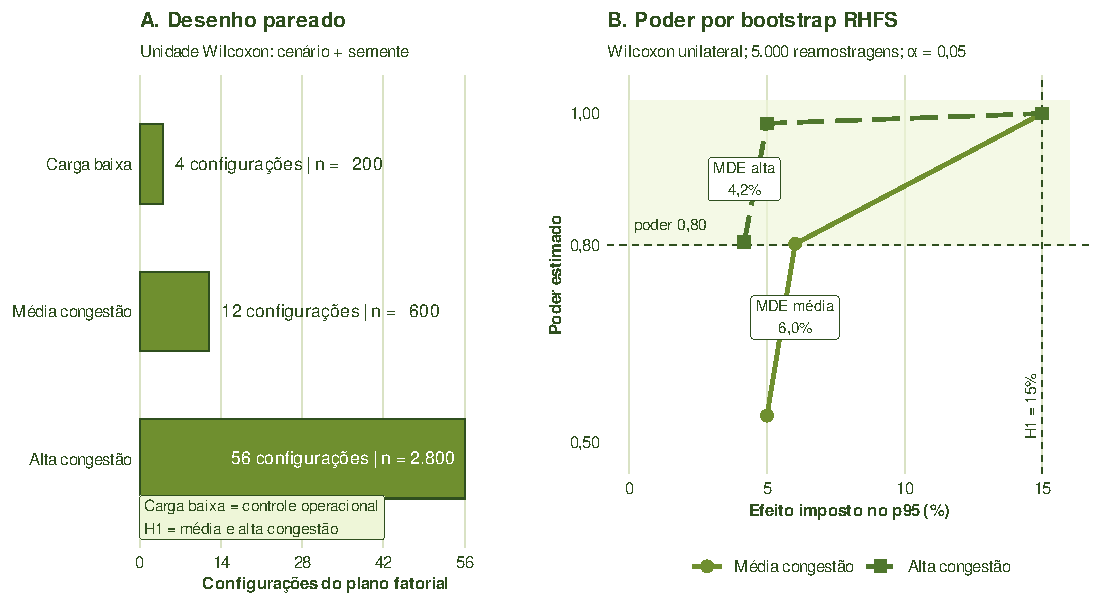
\includegraphics[width=\textwidth]{images/figura-poder-protocolo.pdf}
\caption[Desenho estat\'istico e an\'alise de poder]{Desenho estat\'istico e an\'alise de poder do protocolo confirmat\'orio. O painel A mostra o $n$ efetivo por estrato, calculado como configura\c{c}\~oes $\times$ 50 sementes pareadas. O painel B mostra pontos de refer\^encia do bootstrap sobre a matriz auxiliar RHFS, com Wilcoxon unilateral em $\alpha=0{,}05$.}
\label{fig:desenho-poder-pt}
\end{figure}

Os limiares de 15\% (redu\c{c}\~ao m\'inima do p95, crit\'erio de H1) e 100\% (cobertura de justificativa leg\'ivel, crit\'erio de A2) ser\~ao tratados como metas iniciais acima do ru\'ido operacional esperado. Os valores de $H_0=6$ e dos limiares $\tau_2=10$, $\tau_1=30$, $\tau_0=60$ s\~ao \textbf{pr\'e-especificados} e permanecem fixos no experimento principal; taxas de evento e o multiplicador dos limiares de prioridade ser\~ao verificados na grade de sensibilidade multivariada, sem recalibrar o artefato.

O protocolo inferencial ser\'a hierarquizado. A m\'etrica prim\'aria confirmat\'oria \'e o p95 de espera nos estratos de m\'edia e alta congest\~ao, analisados separadamente. Para cada par formado por estrato $s$ e comparador operacional prim\'ario $c$, a decis\~ao \'e um teste interse\c{c}\~ao--uni\~ao (IUT): o teste unilateral do ganho em p95 deve sustentar a redu\c{c}\~ao m\'inima de 15\%, e a guarda de throughput deve sustentar n\~ao inferioridade contra a margem $\max(2,\;0{,}02N)$ caminh\~oes/dia. A margem de n\~ao inferioridade \'e espec\'ifica de cada configura\c{c}\~ao, calculada como $\delta(N)=\max(2;\,0{,}02N)$ a partir do volume $N$ daquela configura\c{c}\~ao. Para evitar que o agrupamento de configura\c{c}\~oes com $N$ distintos dentro de um estrato misture margens heterog\^eneas, a guarda de throughput \'e testada sobre a diferen\c{c}a pareada deslocada $d'_i=(TH_{\mathrm{Motor},i}-TH_{\mathrm{comp},i})+\delta(N_i)$, aplicando-se o Wilcoxon unilateral a $H_0:\operatorname{mediana}(d')\leq 0$ contra $H_1:\operatorname{mediana}(d')>0$. Assim, cada par contribui com sua pr\'opria margem e o teste do estrato opera sobre uma escala homog\^enea de n\~ao inferioridade. Essa combina\c{c}\~ao de superioridade em uma medida e n\~ao inferioridade em outra segue o uso de IUT para decis\~oes conjuntivas em problemas de equival\^encia e n\~ao inferioridade \parencite{bergerBioequivalenceTrialsIntersectionUnion1996}.

No n\'ivel do estrato, o artefato s\'o ``vence'' se a decis\~ao IUT passar contra os tr\^es comparadores prim\'arios: FIFO \textit{flow-faithful}, prioridade + factibilidade local e despacho din\^amico por escore fixo. Como um IUT decide pela alternativa global apenas quando todos os testes componentes rejeitam, o tamanho do teste global fica no m\'aximo em $\alpha$; a l\'ogica remonta \`a formula\c{c}\~ao de \textcite{bergerMultiparameterHypothesisTesting1982} para testes multiparam\'etricos e amostragem de aceita\c{c}\~ao. Portanto, n\~ao haver\'a corre\c{c}\~ao de multiplicidade entre os tr\^es comparadores prim\'arios dentro de um estrato.

A multiplicidade confirmat\'oria remanescente est\'a entre as duas afirma\c{c}\~oes cient\'ificas substantivas: H1 em m\'edia congest\~ao e H1 em alta congest\~ao. Para essa fam\'ilia de duas hip\'oteses de estrato, o p-valor global de cada estrato ser\'a calculado como o maior p-valor dos componentes exigidos pelo IUT, isto \'e,
\[
p^{\mathrm{IUT}}_{s}=\max_{c \in \mathcal{C}_{\mathrm{prim}}}\left\{p^{\mathrm{p95}}_{s,c},\,p^{\mathrm{thr}}_{s,c}\right\},
\]
e somente os dois valores $\{p^{\mathrm{IUT}}_{\mathrm{med}}, p^{\mathrm{IUT}}_{\mathrm{alta}}\}$ ser\~ao ajustados pelo procedimento sequencial de Holm \parencite{holmSimpleSequentiallyRejective1979}. As demais m\'etricas entram como evid\^encia secund\'aria descritiva.

\begin{table}[H]
\centering
\small
\setlength{\tabcolsep}{6pt}
\renewcommand{\arraystretch}{1.15}
\begin{tabularx}{\textwidth}{@{}P{0.27\textwidth}P{0.25\textwidth}Y@{}}
\toprule
\rowcolor{tablehead}
\textbf{Par\^ametro congelado} & \textbf{Valor inicial} & \textbf{Observa\c{c}\~ao metodol\'ogica} \\
\midrule
Janela ordin\'aria & $H_0=6$, com expans\~ao cr\'itica por limiar de espera & preserva decis\~ao local audit\'avel sem transformar o artefato em escalonador global \\
\addlinespace
Limiares de prioridade & $\tau_2=10$ min, $\tau_1=30$ min, $\tau_0=60$ min & fixos no experimento principal; o multiplicador de estresse entra apenas na sensibilidade \\
\addlinespace
Tratamento de empate num\'erico & normaliza\c{c}\~ao degenerada igual a 0; afinidade imediata bin\'aria & evita divis\~ao indefinida e impede vantagem artificial em filas vazias ou recursos homog\^eneos \\
\addlinespace
Desempate e replay & prioridade, chegada \`a etapa e identificador do caminh\~ao & garante determinismo e reconstruibilidade \\
\bottomrule
\end{tabularx}
\caption[Par\^ametros da pol\'itica de despacho]{Par\^ametros congelados da pol\'itica de despacho.}
\label{tab:parametros-politica}
\end{table}

\noindent\textbf{Nota sobre $H_0$.}
O valor $H_0=6$ \'e tratado como par\^ametro estrutural da pol\'itica, n\~ao calibrado por desempenho, e n\~ao representa otimalidade global. Ele \'e defens\'avel por tr\^es raz\~oes. Primeiro, preserva a no\c{c}\~ao de decis\~ao local e audit\'avel: o auditor reconstr\'oi por que o sistema escolheu um caminh\~ao entre uma vizinhan\c{c}a curta de candidatos ordin\'arios, dialogando com o crit\'erio~A2. Segundo, limita a profundidade de reordena\c{c}\~ao ordin\'aria, evitando que o motor busque caminh\~oes muito atr\'as na fila e gere uma pol\'itica operacionalmente agressiva. Terceiro, gra\c{c}as \`a expans\~ao por press\~ao positiva da Equa\c{c}\~ao~\eqref{eq:cadm}, $H_0$ n\~ao constitui barreira contra urg\^encia: candidatos j\'a cr\'iticos entram no dom\'inio independentemente de sua posi\c{c}\~ao de chegada. A robustez da escolha ser\'a verificada por diagn\'ostico de ativa\c{c}\~ao da janela reportado no Ap\^endice~\ref{apx:material-suplementar} e por sensibilidade em $H_0 \in \{4,6,8\}$ no teste multivariado de estresse, mantida a mesma regra de expans\~ao cr\'itica.

\noindent\textbf{Nota sobre $\tau$ e o multiplicador de estresse.}
Os limiares $\tau_2=10$ min, $\tau_1=30$ min e $\tau_0=60$ min seguem plausibilidade operacional: prioridade alta tolera espera curta, carga padr\~ao tolera espera moderada e carga n\~ao cr\'itica pode aguardar at\'e o fim do turno. Eles permanecem fixos no experimento principal. O multiplicador $\in\{0{,}75;1{,}00;1{,}25\}$ desloca os limiares globalmente na an\'alise de robustez sem alterar a l\'ogica interna do despachante.

O protocolo inclui ainda um \textbf{teste multivariado de estresse}, executado \textbf{ap\'os} o experimento principal e distinto do piloto de sanidade. A grade cruza $H_0 \in \{4,6,8\}$, buffer $\in \{8,12,16\}$, multiplicador dos limiares de prioridade $\in \{0{,}75,1{,}00,1{,}25\}$ e intensidade de eventos $\in \{\text{base},\text{alta}\}$, mantendo a mesma regra de expans\~ao cr\'itica da Equa\c{c}\~ao~\eqref{eq:cadm}. H1 ser\'a tratada como robusta se o artefato preservar ganho mediano positivo no p95 contra todos os comparadores operacionais prim\'arios em pelo menos 75\% da grade, sem violar a margem de throughput.

A rastreabilidade m\'inima dos fatos operacionais usados na pesquisa est\'a consolidada na Tabela~\ref{tab:rastreabilidade-fatos}, no Ap\^endice~\ref{apx:material-suplementar}. No protocolo, esses fatos funcionam como entradas congeladas: orientam filtros de factibilidade, bloqueios, prioridades e requisitos de governan\c{c}a antes da abertura dos resultados.

\section{Métricas e Políticas de Comparação}\label{ch:avaliacao}
\begin{table}[H]
\centering
\small
\setlength{\tabcolsep}{5pt}
\renewcommand{\arraystretch}{1.18}
\begin{tabularx}{\textwidth}{@{}P{0.24\textwidth}P{0.33\textwidth}Y@{}}
\toprule
\rowcolor{tablehead}
\textbf{M\'etrica} & \textbf{Defini\c{c}\~ao operacional} & \textbf{Papel no experimento} \\
\midrule
Espera acumulada em fila & soma, nas quatro etapas, do intervalo entre elegibilidade e in\'icio de servi\c{c}o; reportada por p50 e p95 & m\'etrica prim\'aria confirmat\'oria para H1 \\
\addlinespace
Throughput & caminh\~oes que completam o ciclo no horizonte di\'ario; remanescentes entram como fila final & guarda de n\~ao piora para evitar ganho aparente por abandono de ve\'iculos \\
\addlinespace
Tempo total no sistema & intervalo entre chegada ao p\'atio e conclus\~ao da pesagem final & evid\^encia secund\'aria de experi\^encia operacional por caminh\~ao \\
\addlinespace
Makespan & intervalo entre a primeira chegada e a \'ultima conclus\~ao registrada no dia & verifica alongamento ou compress\~ao do ciclo operacional completo \\
\addlinespace
Utiliza\c{c}\~ao e ociosidade & tempo ocupado por recurso sobre horizonte dispon\'ivel e horizonte bruto; ociosidade como complemento da utiliza\c{c}\~ao l\'iquida & contrapartida de capacidade para interpretar redu\c{c}\~oes de fila \\
\addlinespace
Estabilidade e reordena\c{c}\~ao & invers\~oes entre filas consecutivas, quebra de FIFO e frequ\^encia de replanejamento & mede custo decis\'orio e ader\^encia operacional \\
\addlinespace
Factibilidade e justificativa leg\'ivel & atendimento das restri\c{c}\~oes r\'igidas e presen\c{c}a dos campos de auditoria definidos na Se\c{c}\~ao~\ref{ch:artefato} & valida seguran\c{c}a, governan\c{c}a e reconstruibilidade \\
\addlinespace
$\mathrm{CO_2}$ estimado & emiss\~ao derivada do tempo em fila com motor ligado, usando consumo em marcha lenta e fator de emiss\~ao declarados & indicador explorat\'orio, sem papel confirmat\'orio \\
\bottomrule
\end{tabularx}
\caption[M\'etricas do simulador]{M\'etricas consolidadas do simulador e papel experimental.}
\label{tab:metricas-consolidadas}
\end{table}

O indicador ambiental usa a fronteira de motor ligado em fila e entra apenas como vari\'avel derivada. A redu\c{c}\~ao de tempo em marcha lenta (\textit{idle time}) \'e adotada como m\'etrica operacional de iniciativas verdes em agendamento de caminh\~oes, conforme o tratamento de custos e emiss\~oes por ociosidade em \textcite{liDisruptionManagementTruck2018a}. Para a pol\'itica $\pi$, calcula-se $\widehat{E}_{\mathrm{CO_2}}(\pi)=\left(\sum_{i \in I} W_i^{\mathrm{fila}}(\pi)/60\right)\rho_{\mathrm{idle}}\gamma_{\mathrm{diesel}}$, com $\rho_{\mathrm{idle}}=0{,}8$ gal\~ao/hora no valor-base, sensibilidade em $[0{,}5;\,1{,}0]$ gal\~ao/hora e $\gamma_{\mathrm{diesel}}=10{,}18$ kg $\mathrm{CO_2}$/gal\~ao \parencite{usdoeIdleFuelConsumption2015, usepaGreenhouseGasEquivalencies2026}. Deslocamento, partida a frio, poeira, eletricidade e ciclo de vida do combust\'ivel ficam fora do c\'alculo.

O conjunto de compara\c{c}\~ao re\'une quatro pol\'iticas de refer\^encia e o artefato proposto. FIFO e BATCH aparecem em recebimento de gr\~aos como regras simples \parencite{r.berrutoAnalyzingReceivingOperation2001a}; appointment systems e agendamento colaborativo refor\c{c}am compara\c{c}\~oes al\'em do FIFO \parencite{phanCollaborativeTruckScheduling2016a, azabDynamicCollaborativeTruck2017a}; e trabalhos de disrup\c{c}\~ao/reagendamento separam resposta a eventos de plano est\'atico inicial \parencite{liDisruptionManagementTruck2018a, xuDynamicAppointmentRescheduling2022}. O escore fixo \'e um advers\'ario din\^amico cr\'ivel: uma regra de \'indice ponderado inspirada nas regras de despacho composto (\textit{composite dispatching rules}) catalogadas por \textcite{panwalkarSurveySchedulingRules1977} e na fam\'ilia ATC/COVERT estudada por \textcite{vepsalainenPriorityRulesJob1987}. A Tabela~\ref{tab:politicas-experimento} fixa o papel de cada pol\'itica; as pol\'iticas deslocadas para sensibilidade aparecem no Ap\^endice~\ref{apx:politicas-secundarias}.

\begin{table}[H]
\centering
\small
\setlength{\tabcolsep}{6pt}
\renewcommand{\arraystretch}{1.15}
\begin{tabularx}{\textwidth}{@{}P{0.23\textwidth}P{0.33\textwidth}Y@{}}
\toprule
\rowcolor{tablehead}
\textbf{Pol\'itica} & \textbf{Regra congelada} & \textbf{Papel na compara\c{c}\~ao} \\
\midrule
FIFO estrito & atende por chegada \`a etapa; se o primeiro caminh\~ao estiver ineleg\'ivel, o recurso aguarda ou registra bloqueio & limite inferior descritivo, fora do teste substantivo de H1 \\
\addlinespace
FIFO \textit{flow-faithful} & escolhe o candidato mais antigo dentro de $C^{adm}_{k,r}$ & comparador operacional prim\'ario baseado em FIFO fact\'ivel \\
\addlinespace
Prioridade + factibilidade local & ordena $C^{adm}_{k,r}$ por prioridade operacional e chegada \`a etapa & comparador prim\'ario para medir ganho al\'em de prioridade e factibilidade \\
\addlinespace
Despacho din\^amico por escore fixo & aplica $0{,}45$ espera normalizada $+0{,}35$ prioridade $+0{,}20$ afinidade imediata & comparador din\^amico principal, pr\'e-especificado e sem calibra\c{c}\~ao pelo piloto \\
\addlinespace
Artefato proposto & aplica ranking lexicogr\'afico $h_{k,r}(i)$, desempates fixos e registro audit\'avel & pol\'itica principal da pesquisa \\
\bottomrule
\end{tabularx}
\caption[Pol\'iticas do experimento principal]{Pol\'iticas do experimento principal. H1 ser\'a julgada contra FIFO \textit{flow-faithful}, prioridade + factibilidade local e despacho din\^amico por escore fixo.}
\label{tab:politicas-experimento}
\end{table}

Como fixado na Se\c{c}\~ao~\ref{sec:formulacao-despacho}, as pol\'iticas do painel confirmat\'orio observar\~ao a mesma verdade local validada, a mesma checagem de restri\c{c}\~oes r\'igidas, o mesmo dom\'inio admiss\'ivel, o mesmo bloqueio formal e o mesmo log. Varia somente a regra de sele\c{c}\~ao quando h\'a mais de uma alternativa eleg\'ivel; factibilidade, admiss\~ao e registro pertencem \`a plataforma experimental, n\~ao a uma vantagem exclusiva do artefato.

O prot\'otipo registrar\'a, por decis\~ao, entradas consideradas, restri\c{c}\~oes ativadas, alternativa selecionada, eventual quebra de FIFO e interven\c{c}\~ao manual. `Justificativa leg\'ivel` exige cinco campos: caminh\~ao/etapa, recurso escolhido ou bloqueado, regras ativadas, motivo da decis\~ao e quebra de FIFO. Esse registro permite reconstruir a decis\~ao depois da execu\c{c}\~ao, inclusive quando o operador aceita uma recomenda\c{c}\~ao, altera a sequ\^encia ou mant\'em o recurso bloqueado. A governan\c{c}a humana segue tr\^es regras: s\'o perfis autorizados interv\^em, toda interven\c{c}\~ao tem motivo textual e nenhuma sobreposi\c{c}\~ao viola restri\c{c}\~oes r\'igidas. A literatura de rastreabilidade digital no p\'os-colheita apoia a dimens\~ao de auditoria \parencite{dyckDigitalTwinsNovel2023}.

A avalia\c{c}\~ao executa o protocolo deste cap\'itulo, com as m\'etricas consolidadas na Tabela~\ref{tab:metricas-consolidadas}. O \textbf{Bloco A} compara pol\'iticas em cen\'arios simulados; o \textbf{Bloco B} audita seguran\c{c}a operacional e rastreabilidade do artefato. Todos os comparadores usar\~ao o mesmo simulador, eventos, filtro de factibilidade, logs e sementes; muda somente a pol\'itica de ranqueamento/sele\c{c}\~ao.

O Bloco A compara cen\'arios equivalentes, executando cada cen\'ario com todas as pol\'iticas. A literatura aponta maior fragilidade de regras est\'aticas sob variabilidade e press\~ao sobre recursos \parencite{abdelmagidComprehensiveReviewTruck2022a, nasiriPredictivereactiveCrossdockRescheduling2022, wangFlexibleStorageYard2023}. A m\'etrica confirmat\'oria ser\'a o p95 da \textbf{espera acumulada em fila}; throughput atuar\'a como guarda de n\~ao piora. Tempo total no sistema, makespan, estabilidade, viola\c{c}\~oes evit\'aveis de FIFO, utiliza\c{c}\~ao l\'iquida/bruta, ociosidade e $\mathrm{CO_2}$ estimado ser\~ao secund\'arias. A estimativa ambiental n\~ao adiciona uma segunda prova de desempenho: ela traduz, em unidade f\'isica, a espera com motor ligado. Para mitigar vi\'es de agrega\c{c}\~ao, resultados de espera nunca ser\~ao apresentados apenas como m\'edia global dos 72 cen\'arios; toda tabela ou figura de desempenho dever\'a separar \textbf{carga baixa}, \textbf{m\'edia congest\~ao} e \textbf{alta congest\~ao}.

H1 exige redu\c{c}\~ao de pelo menos 15\% na mediana pareada do p95 da espera acumulada em fila, nos estratos de m\'edia e alta congest\~ao analisados separadamente, contra FIFO \textit{flow-faithful}, prioridade + factibilidade local e despacho din\^amico por escore fixo. O artefato tamb\'em deve respeitar a margem protetiva de throughput $\max(2,\;0{,}02N)$ caminh\~oes/dia. Assim, a decis\~ao confirmat\'oria passa por duas conjun\c{c}\~oes: dentro de cada par comparador--estrato, p95 e throughput precisam passar; dentro de cada estrato, os tr\^es comparadores prim\'arios precisam passar. No Bloco B, A1 ser\'a verificado por validador determin\'istico independente, inclusive em casos adversariais; A2 ser\'a verificado por completude e reconstruibilidade dos logs, com cobertura estrutural de 100\% e amostra auditada.

O protocolo separa fatos operacionais, hip\'oteses de calibra\c{c}\~ao e resultados observados. Al\'em do Wilcoxon signed-rank, o estudo reportar\'a mediana e IQR das diferen\c{c}as pareadas, Hodges--Lehmann, bootstrap pareado de 95\% e $r_{rb}$. Empates e diferen\c{c}as zero ser\~ao explicitados; se dominarem, o teste de sinais pareado entrar\'a como robustez. Cen\'arios de desenvolvimento, piloto e experimento principal permanecem separados quanto ao prop\'osito (sanidade vs. confirma\c{c}\~ao), sem que ajustes do piloto retroajam sobre os par\^ametros congelados.

O piloto verificar\'a sanidade das m\'etricas e do simulador, estabilidade do ganho pareado no p95 e aus\^encia de comportamento degenerado. A estabilidade ser\'a observada pela largura do intervalo bootstrap de 95\% para a melhoria mediana e pelo IQR do ganho pareado. O n\'umero de sementes permanece fixo em 50. O piloto mant\'em $H$, limiares $\tau$ e pesos $(0{,}45;\,0{,}35;\,0{,}20)$ pr\'e-especificados, de modo que a compara\c{c}\~ao principal avalie par\^ametros congelados, sem ajuste conjunto.

A unidade de an\'alise fica congelada: decis\~oes individuais alimentam auditoria; m\'etricas por caminh\~ao geram resumos por dia simulado; m\'etricas de equipamento agregam por recurso e classe, preservando portaria, balan\c{c}as e moegas como categorias separadas. O Wilcoxon ser\'a aplicado sobre pares `cen\'ario + semente`, com uma observa\c{c}\~ao por dia e pol\'itica, separada por estrato de congest\~ao. O ajuste de Holm incidir\'a somente sobre os dois p-valores globais de estrato calculados pela l\'ogica IUT; n\~ao ser\'a aplicado aos tr\^es comparadores prim\'arios nem \`as m\'etricas secund\'arias. A carga baixa ser\'a reportada como estrato de controle operacional, sem expectativa confirmat\'oria de superioridade; m\'edia e alta congest\~ao formam os estratos substantivos de H1. Qualquer agregado geral, se inclu\'ido, ter\'a car\'ater meramente descritivo e dever\'a aparecer depois dos resultados estratificados.

Uma amostra de $\max(50,\;10\%)$ das decis\~oes do artefato por cen\'ario ser\'a auditada por rubrica fechada, al\'em da checagem autom\'atica de 100\% dos logs. A rubrica verifica campos obrigat\'orios, regra ativada, quebra de FIFO, a\c{c}\~ao humana admiss\'ivel e reconstru\c{c}\~ao do estado. Quando houver dois avaliadores, ser\'a reportado kappa de Cohen; concord\^ancia abaixo de 0,60 exigir\'a revis\~ao da rubrica antes do congelamento final.

\subsection{Disponibilidade de Dados e Código}\label{sec:disponibilidade-dados-codigo}
Os dados sint\'eticos, sementes, inst\^ancias, logs agregados, sa\'idas experimentais, scripts de an\'alise e c\'odigo-fonte customizado necess\'arios para reproduzir os resultados da etapa experimental posterior ser\~ao disponibilizados em reposit\'orio p\'ublico ou m\'idia institucional no momento da entrega final, sujeitos a restri\c{c}\~oes institucionais. A vers\~ao utilizada na an\'alise ser\'a identificada por URL, tag ou hash de commit, com instru\c{c}\~oes de execu\c{c}\~ao, vers\~oes de depend\^encias e ambiente computacional.

Este reposit\'orio do TCC, em especial \texttt{main.tex} e \texttt{refs.bib}, \'e a
\textbf{fonte can\^onica} da terminologia, dos par\^ametros, das tabelas e do protocolo.
Reposit\'orios de implementa\c{c}\~ao podem manter c\'opias geradas para reprodu\c{c}\~ao,
mas n\~ao podem redefinir o protocolo. Cada execu\c{c}\~ao dever\'a registrar o hash da
vers\~ao can\^onica usada, o checksum dos par\^ametros e o esquema dos eventos exportados ao
modelo digital.

Dados reais, documentos sens\'iveis ou informa\c{c}\~oes operacionais identific\'aveis n\~ao ser\~ao inclu\'idos no pacote aberto. Quando algum artefato n\~ao puder ser disponibilizado integralmente, ser\'a fornecida vers\~ao sint\'etica ou anonimizada com a mesma estrutura de campos e diferen\c{c}as declaradas. At\'e a libera\c{c}\~ao final do reposit\'orio congelado, os materiais de reprodu\c{c}\~ao ficam dispon\'iveis mediante solicita\c{c}\~ao razo\'avel ao autor.

\chapter{Resultados Parciais}

Nesta etapa, ``resultado'' n\~ao significa ainda superioridade estat\'istica do motor. O resultado do TCC~I \'e a prepara\c{c}\~ao verific\'avel do experimento: recorte operacional definido, restri\c{c}\~oes r\'igidas explicitadas, pol\'iticas de refer\^encia congeladas, par\^ametros sint\'eticos justificados, m\'etricas selecionadas e protocolo estat\'istico descrito. A compara\c{c}\~ao principal de desempenho permanece reservada ao TCC~II; o que se demonstra aqui \'e a exist\^encia de uma base implementada e test\'avel, ainda sujeita \`a execu\c{c}\~ao confirmat\'oria e \`a valida\c{c}\~ao de face previstas.

\section{Dados, tratamento e preparação experimental}

Os dados principais s\~ao sint\'eticos, parametrizados e controlados. Essa escolha isola o efeito da pol\'itica de despacho, permite pareamento por sementes e garante reprodutibilidade. Dados reais ampliariam a validade externa, mas tamb\'em trariam heterogeneidade operacional e restri\c{c}\~oes de acesso que extrapolam a etapa atual.

O tratamento experimental j\'a est\'a especificado no Cap\'itulo~\ref{ch:metodologia}: plano fatorial, par\^ametros sint\'eticos, hip\'oteses congeladas, plausibilidade dos par\^ametros, limiares da pol\'itica e pol\'iticas de compara\c{c}\~ao. Nesta etapa, o resultado parcial relevante \'e a consolida\c{c}\~ao desse protocolo em uma trilha reprodut\'ivel, na qual cada dia simulado possui cen\'ario, semente, pol\'itica e sa\'idas agregadas identific\'aveis.

O experimento principal comparativo, descrito nas matrizes da Se\c{c}\~ao~4.2, ser\'a executado no TCC~II. O motor e o simulador possuem implementa\c{c}\~ao preliminar em reposit\'orio adjacente, com testes automatizados e execu\c{c}\~oes parciais de desenvolvimento; isso demonstra implementabilidade, n\~ao desempenho confirmat\'orio. Um auditor independente dos artefatos persistidos verifica A1, completude estrutural de A2, hashes e consist\^encia entre CSV e JSONL; sua aplica\c{c}\~ao \`a matriz completa e a inspe\c{c}\~ao humana da amostra A2 ainda precisam ser realizadas. Tamb\'em permanecem pendentes as 18.000 execu\c{c}\~oes e a an\'alise de H1. O projeto Unreal Engine~5.8 est\'a inicializado, mas ainda n\~ao cont\'em a cena de dom\'inio nem o replay integrado. A Tabela~\ref{tab:resultados-repos-adjacentes}, no Ap\^endice~\ref{apx:materiais-contextuais}, registra apenas evid\^encias auxiliares e seus limites \parencite{hevnerDesignScienceInformation2004a}.

\section{Matriz de resultados prevista para o TCC~II}

Os resultados quantitativos do TCC~II ser\~ao apresentados apenas ap\'os a execu\c{c}\~ao consolidada do simulador. Nesta vers\~ao, o corpo do texto evita tabelas vazias e registra somente a l\'ogica de leitura: H1 ser\'a julgada pela redu\c{c}\~ao pareada do p95 de espera acumulada, preservada a margem protetiva de throughput, nos estratos de m\'edia e alta congest\~ao.

As matrizes tabulares previstas para o TCC~II foram deslocadas para as Tabelas~\ref{tab:gap-espera-p95-previsto}, \ref{tab:diag-h} e~\ref{tab:estabilidade-prioridade-prevista}, no Ap\^endice~\ref{apx:material-suplementar}. Elas definem campos a preencher apenas depois da execu\c{c}\~ao do simulador, preservando a separa\c{c}\~ao entre carga baixa, m\'edia congest\~ao e alta congest\~ao. A Figura~\ref{fig:throughput-espera-prevista} permanece no corpo como esquema visual de leitura entre throughput e espera.

\begin{figure}[H]
\centering
\resizebox{0.80\textwidth}{!}{%
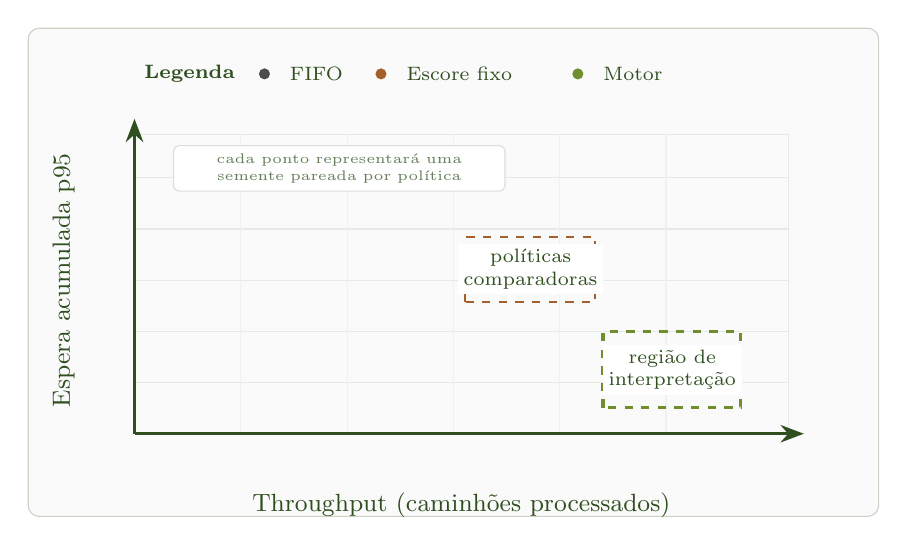
\begin{tikzpicture}[font=\small, >=Stealth]
  \fill[gray!4, rounded corners=4pt] (0,0) rectangle (10.8,6.2);
  \draw[pequiDark!25, rounded corners=4pt] (0,0) rectangle (10.8,6.2);

  \draw[pequiDark!12] (1.35,1.05) rectangle (9.65,4.85);
  \foreach \y in {1.70,2.35,3.00,3.65,4.30} {
    \draw[pequiDark!12] (1.35,\y) -- (9.65,\y);
  }
  \foreach \x in {2.70,4.05,5.40,6.75,8.10} {
    \draw[pequiDark!8] (\x,1.05) -- (\x,4.85);
  }

  \draw[->, very thick, pequiDark] (1.35,1.05) -- (9.85,1.05);
  \draw[->, very thick, pequiDark] (1.35,1.05) -- (1.35,5.05);
  \node[below, text=pequiDark] at (5.50,0.42) {Throughput (caminh\~oes processados)};
  \node[rotate=90, text=pequiDark] at (0.45,3.00) {Espera acumulada p95};
  \node[font=\scriptsize\bfseries, text=pequiDark, anchor=west] at (1.35,5.62) {Legenda};
  \fill[black!70] (3.00,5.62) circle (2pt);
  \node[font=\scriptsize, text=pequiDark, anchor=west] at (3.20,5.62) {FIFO};
  \fill[pequiEarth] (4.48,5.62) circle (2pt);
  \node[font=\scriptsize, text=pequiDark, anchor=west] at (4.68,5.62) {Escore fixo};
  \fill[pequiGreen] (6.98,5.62) circle (2pt);
  \node[font=\scriptsize, text=pequiDark, anchor=west] at (7.18,5.62) {Motor};

  \node[align=center, text width=4.0cm, font=\tiny, text=pequiDark!75,
        fill=white, draw=pequiDark!18, rounded corners=2pt, inner sep=3pt] at (3.95,4.42)
    {cada ponto representar\'a uma\\
     semente pareada por pol\'itica};

  \draw[pequiEarth, thick, dashed] (5.55,2.72) rectangle (7.20,3.55);
  \node[font=\scriptsize, align=center, text=pequiDark,
        fill=white, inner sep=2pt] at (6.38,3.14) {pol\'iticas\\comparadoras};

  \draw[pequiGreen, very thick, dashed] (7.30,1.38) rectangle (9.05,2.35);
  \node[font=\scriptsize, align=center, text=pequiDark,
        fill=white, inner sep=2pt] at (8.18,1.86) {regi\~ao de\\interpreta\c{c}\~ao};
\end{tikzpicture}%
}
\caption[Leitura conjunta de throughput e espera]{Leitura conjunta prevista para throughput e espera acumulada p95. Cada ponto representar\'a uma semente pareada de uma pol\'itica no TCC~II; a regi\~ao indicada funciona apenas como guia para interpretar menor espera sem recuo material de throughput, n\~ao como resultado antecipado.}
\label{fig:throughput-espera-prevista}
\end{figure}

\chapter{Cronograma}

O cronograma traduz o protocolo em uma sequ\^encia de trabalho para o TCC~II. A ordem das macroetapas preserva as depend\^encias principais: fechamento de protocolo, implementa\c{c}\~ao e valida\c{c}\~ao, execu\c{c}\~ao experimental, an\'alise, reda\c{c}\~ao e defesa.

\begin{table}[H]
\centering
\setlength{\tabcolsep}{3pt}
\scriptsize
\renewcommand{\arraystretch}{1.15}
\begin{tabular}{@{}P{0.34\textwidth}*{7}{C{0.06\textwidth}}@{}}
\toprule
\rowcolor{tablehead}
\textbf{Macroetapa} & \shortstack{\textbf{Jun.}\\\textbf{26}} & \shortstack{\textbf{Jul.}\\\textbf{26}} & \shortstack{\textbf{Ago.}\\\textbf{26}} & \shortstack{\textbf{Set.}\\\textbf{26}} & \shortstack{\textbf{Out.}\\\textbf{26}} & \shortstack{\textbf{Nov.}\\\textbf{26}} & \shortstack{\textbf{Dez.}\\\textbf{26}} \\
\midrule
Fechamento de escopo, literatura e protocolo & \timeline & \timeline &  &  &  &  &  \\
Implementa\c{c}\~ao do simulador, logs e validadores &  & \timeline & \timeline & \timeline &  &  &  \\
Desenvolvimento do modelo digital no Unreal Engine~5.8 &  & \timeline & \timeline & \timeline & \timeline &  &  \\
Gera\c{c}\~ao de cen\'arios, piloto e congelamento de par\^ametros &  &  & \timeline & \timeline &  &  &  \\
Execu\c{c}\~ao do experimento principal &  &  &  &  & \timeline & \timeline &  \\
An\'alise estat\'istica, sensibilidade e auditoria dos logs &  &  &  &  &  & \timeline & \timeline \\
Reda\c{c}\~ao dos resultados, discuss\~ao e conclus\~ao &  &  &  & \timeline & \timeline & \timeline & \timeline \\
Revis\~ao final, apresenta\c{c}\~ao e defesa &  &  &  &  &  & \timeline & \timeline \\
\bottomrule
\end{tabular}
\caption[Cronograma da pesquisa]{Cronograma macro de execu\c{c}\~ao da pesquisa entre junho e dezembro de 2026.}
\label{tab:cronograma-pesquisa}
\end{table}

\chapter{Ameaças à validade}
Mesmo com protocolo fechado, o desenho experimental ainda pode falhar em pontos espec\'ificos. O primeiro risco \'e de constru\c{c}\~ao: uma ``justificativa leg\'ivel'' pode registrar a regra acionada sem realmente ajudar o avaliador a entender a decis\~ao. A mitiga\c{c}\~ao combina rubrica fechada, inspe\c{c}\~ao humana e checagem de campos obrigat\'orios. O segundo risco \'e interno: par\^ametros calibrados a favor do artefato poderiam inflar o ganho observado. Para reduzir esse vi\'es, requisitos, pol\'iticas de refer\^encia e par\^ametros do simulador ficam separados, e as compara\c{c}\~oes usam sementes pareadas, margem de throughput e teste multivariado de estresse. Tamb\'em h\'a risco de implementa\c{c}\~ao; erros no simulador poderiam favorecer uma pol\'itica. Por isso, o protocolo exige validadores determin\'isticos, logs por evento e replay audit\'avel das restri\c{c}\~oes r\'igidas.

A validade externa delimita o alcance dos resultados: cen\'arios sint\'eticos calibrados sustentam coer\^encia, factibilidade e desempenho comparativo em ambiente controlado; uma cooperativa espec\'ifica exige dados locais. Valida\c{c}\~ao de face, plausibilidade param\'etrica e registro de diverg\^encias conectam o modelo sint\'etico ao dom\'inio operacional.

O modelo digital em Unreal Engine introduz uma amea\c{c}a adicional de validade de
representa\c{c}\~ao: anima\c{c}\~ao visual plaus\'ivel pode sugerir fidelidade operacional que
os dados sint\'eticos n\~ao sustentam. A mitiga\c{c}\~ao consiste em reproduzir somente
estados presentes no log can\^onico, validar o esquema de interc\^ambio e identificar a cena
como modelo digital de pesquisa. Sem telemetria de ativo f\'isico e sincroniza\c{c}\~ao
bidirecional, nenhum resultado ser\'a descrito como valida\c{c}\~ao de g\^emeo digital.

A discretiza\c{c}\~ao de $\rho$ implica que o estrato de m\'edia congest\~ao repousa sobre um \'unico n\'ivel nominal de carga ($\rho=0{,}833$); a evid\^encia de H1 nesse estrato apoia-se na varia\c{c}\~ao do recurso ligante entre as tr\^es configura\c{c}\~oes, e n\~ao em uma faixa cont\'inua de carga. A extrapola\c{c}\~ao para cargas intermedi\'arias n\~ao amostradas ($0{,}85 \leq \rho < 1{,}11$) permanece fora do escopo confirmat\'orio.

A s\'intese de cen\'arios adiciona risco de contamina\c{c}\~ao sem\^antica entre descri\c{c}\~ao operacional, estrutura formal e comportamento simulado. Um cen\'ario pode soar plaus\'ivel e ainda assim representar outro problema quando convertido em vari\'aveis, restri\c{c}\~oes e eventos. A mitiga\c{c}\~ao exige estruturas formais, valida\c{c}\~ao determin\'istica, execu\c{c}\~ao no simulador, rejei\c{c}\~ao de inst\^ancias inconsistentes e logs de origem. Se logs reais forem incorporados no futuro, o protocolo dever\'a acrescentar matriz de depend\^encias, cobertura de segmentos raros e avalia\c{c}\~ao de risco de privacidade.

A abstra\c{c}\~ao em quatro etapas delimita a fronteira do modelo e concentra a an\'alise nos gargalos que determinam filas, bloqueios e propaga\c{c}\~ao de atrasos.

Como risco de modelagem estat\'istica de entrada, distribui\c{c}\~oes triangulares n\~ao reproduzem caudas longas \`a direita t\'ipicas de tempos de servi\c{c}o altamente assim\'etricos. Law demonstra que aproximar uma lognormal por uma triangular com m\'inimo e moda corretos pode subestimar severamente a espera m\'edia em fila em um sistema M/G/1 \parencite[Ex.~6.23, p.~376--377]{lawSimulationModelingAnalysis2015}. Nesta pesquisa, esse risco \'e mitigado por eventos disruptivos separados, an\'alise estratificada por congest\~ao, m\'etrica p95 e valida\c{c}\~ao de face; ainda assim, resultados sob disrup\c{c}\~ao extrema devem ser lidos como evid\^encia controlada, n\~ao como previs\~ao de cauda operacional real.

Tamb\'em h\'a amea\c{c}a de validade estat\'istica: a compara\c{c}\~ao envolve m\'ultiplas pol\'iticas, cen\'arios e m\'etricas. O protocolo responde com pareamento por semente, separa\c{c}\~ao entre m\'etrica confirmat\'oria e m\'etricas secund\'arias, decis\~ao IUT para os comparadores prim\'arios e corre\c{c}\~ao de Holm restrita \`as duas hip\'oteses de estrato. Com isso, a interpreta\c{c}\~ao evita transformar cada indicador explorat\'orio em confirma\c{c}\~ao independente sem desperdi\c{c}ar poder com corre\c{c}\~ao sobre uma conjun\c{c}\~ao que j\'a controla o erro.

\chapter{Conclusão}\label{ch:conclusao}
Este trabalho parte de uma decis\~ao simples de enunciar e dif\'icil de executar: quando um recurso fica livre, qual caminh\~ao deve ser atendido a seguir? Ao formular essa escolha como despacho online sob restri\c{c}\~oes, a pesquisa transforma uma pr\'atica operacional muitas vezes t\'acita em artefato computacional model\'avel, audit\'avel e avali\'avel. A revis\~ao de literatura aproxima o problema de truck appointment systems, scheduling sob incerteza e replanejamento em tempo real, mas o contexto agroindustrial imp\~oe condi\c{c}\~oes pr\'oprias: falha segura, bloqueios documentais, chuva, compatibilidade carga--recurso, rastreabilidade e controle humano.

O TCC~I consolida quatro bases para a etapa experimental. A primeira \'e a modelagem formal do problema (Se\c{c}\~ao~\ref{ch:modelagem}), com $S_k$, $C_{k,r}$, $h_{k,r}(i)$ e execu\c{c}\~ao determin\'istica. A segunda \'e o desenho experimental (Cap\'itulo~\ref{ch:metodologia}), com pol\'iticas congeladas, regimes de perturba\c{c}\~ao, estratos de congest\~ao, m\'etricas, limiares de H1/A1/A2 e protocolo estat\'istico. A terceira \'e o plano de reprodutibilidade (Se\c{c}\~ao~\ref{sec:disponibilidade-dados-codigo}), com dados sint\'eticos, sementes, logs, scripts de an\'alise e identifica\c{c}\~ao da vers\~ao por URL, tag ou hash de commit. A quarta \'e a arquitetura do modelo digital no Unreal Engine~5.8, que transforma logs do simulador em visualiza\c{c}\~ao e replay sem assumir o papel de g\^emeo digital.

H1 ser\'a verificada no TCC~II: reduzir em pelo menos 15\% a mediana pareada do p95 da espera acumulada em fila, nos estratos de m\'edia e alta congest\~ao, sem violar a margem protetiva de throughput. A1 e A2 complementam H1 ao separar desempenho de pol\'itica e qualidade de artefato: A1 exige aus\^encia de viola\c{c}\~ao de restri\c{c}\~oes r\'igidas validada independentemente; A2 exige rastreabilidade e reconstruibilidade de decis\~oes e interven\c{c}\~oes humanas.

Quatro fronteiras delimitam as conclus\~oes: cen\'arios sint\'eticos n\~ao substituem valida\c{c}\~ao de campo; par\^ametros dependem de literatura, hip\'oteses de engenharia e valida\c{c}\~ao de face ainda pendente; a decomposi\c{c}\~ao em quatro etapas concentra o modelo nos gargalos de fila, bloqueio e propaga\c{c}\~ao de atrasos; e a representa\c{c}\~ao no Unreal Engine \'e um modelo digital, n\~ao evid\^encia de sincroniza\c{c}\~ao com um sistema f\'isico real.

O trabalho contribui para sistemas de apoio \`a decis\~ao em log\'istica agroindustrial com maior auditabilidade, resposta a eventos disruptivos e supervis\~ao humana. O motor proposto e o modelo digital oferecem uma base reprodut\'ivel para experimenta\c{c}\~ao controlada e futura valida\c{c}\~ao em campo, sem antecipar validade operacional ainda n\~ao demonstrada.

A principal entrega desta etapa, portanto, n\~ao \'e um resultado de superioridade emp\'irica, mas um protocolo fechado para test\'a-la. O TCC~II dever\'a executar esse protocolo, reportar ganhos e perdas por estrato de congest\~ao, auditar logs e discutir os casos em que o artefato n\~ao superar comparadores fortes. Essa delimita\c{c}\~ao preserva a for\c{c}a da contribui\c{c}\~ao: o trabalho apresenta uma formula\c{c}\~ao reprodut\'ivel, comparadores definidos e crit\'erios claros de aceita\c{c}\~ao.

\begin{apendicesenv}

\chapter{Material suplementar de compara\c{c}\~ao e resultados previstos}\label{apx:material-suplementar}

Este ap\^endice re\'une matrizes de apoio que documentam compara\c{c}\~ao com literatura, rastreabilidade de fatos operacionais e formatos previstos de reporte. O conte\'udo \'e suplementar: n\~ao antecipa resultado emp\'irico nem altera os crit\'erios confirmat\'orios de H1, A1 e A2.

\section{Compara\c{c}\~ao direta com a literatura}

{\footnotesize
\setlength{\tabcolsep}{4pt}
\renewcommand{\arraystretch}{1.18}
\begin{longtable}{@{}P{0.18\textwidth}P{0.23\textwidth}P{0.24\textwidth}P{0.25\textwidth}@{}}
\caption[Compara\c{c}\~ao com a literatura]{Compara\c{c}\~ao direta entre motor proposto e frentes da revis\~ao de literatura.}\label{tab:comparacao-literatura}\\
\toprule
\rowcolor{tablehead}
\textbf{Frente} & \textbf{Cobertura da literatura} & \textbf{Similaridade} & \textbf{Diferen\c{c}a e uso na pesquisa} \\
\midrule
\endfirsthead
\toprule
\rowcolor{tablehead}
\textbf{Frente} & \textbf{Cobertura da literatura} & \textbf{Similaridade} & \textbf{Diferen\c{c}a e uso na pesquisa} \\
\midrule
\endhead
TAS & Agendamento de caminh\~oes, janelas, capacidade de port\~ao e congestionamento \parencite{phanCollaborativeTruckScheduling2016a, abdelmagidComprehensiveReviewTruck2022a, graciaTruckAppointmentScheduling2025a, bouyahiaNovelTruckAppointment2025b}. & Coordena caminh\~oes sob capacidade limitada, com espera, throughput e utiliza\c{c}\~ao. & TAS atua antes da chegada ou no port\~ao; o artefato atua como despachante interno online com bloqueios, chuva, compatibilidade e log audit\'avel. \\
\addlinespace
Cross-docking & Sequenciamento, portas, docas, rotas, incerteza e replanejamento \parencite{boysenCrossDockScheduling2010a, cotaIntegratingVehicleScheduling2022, nasiriPredictivereactiveCrossdockRescheduling2022, torbaliMultiagentbasedRealtimeTruck2023, fonsecaStabilityApproachCDC2025}. & Compartilha filas, recursos, preced\^encias, atrasos e reavalia\c{c}\~ao por evento. & Sustenta comparadores din\^amicos e estabilidade, mas o dom\'inio aqui \'e recebimento agroindustrial com segrega\c{c}\~ao de produto. \\
\addlinespace
Elevadores de gr\~aos & Filas, recebimento, mistura de cargas, gargalos e simula\c{c}\~ao discreta \parencite{boulandTruckQueuesCountry1967a, leblancQueuingModelSimulation1978a, r.berrutoAnalyzingReceivingOperation2001a, t.j.herrmanUseSimulationModel2002a, m.e.a.inglesEffectsGrainreceivingSystem2006a, silvaSimulationToolsetModeling2012a, turnerDiscreteEventSimulation2019a, fioroniFarmPortSimulation2015a}. & \'E a frente mais pr\'oxima do dom\'inio por tratar caminh\~oes, gr\~aos e capacidade de recebimento. & Ancora par\^ametros, etapas, FIFO/BATCH e plausibilidade, mas n\~ao entrega motor de despacho online audit\'avel. \\
\addlinespace
DSS & Apoio \`a decis\~ao para carga, recursos, rotas, armazenagem e distribui\c{c}\~ao \parencite{vanderheydenDecisionSupportSystem1985a, hillDecisionSupportSystem2017aa, mardanehDecisionSupportSystem2021a}. & Assume decis\~ao assistida, com supervis\~ao humana. & Justifica explicabilidade e interven\c{c}\~ao humana, enquanto o artefato especifica decis\~ao local por caminh\~ao/etapa. \\
\addlinespace
Modelos digitais e g\^emeos digitais & Representa\c{c}\~ao computacional, estado observ\'avel e integra\c{c}\~ao entre entidades f\'isicas e digitais \parencite{kritzingerDigitalTwinManufacturing2018,dyckDigitalTwinsNovel2023,nistDigitalTwinsEssentialElements2026}. & Exige hist\'orico de eventos e reconstru\c{c}\~ao posterior. & O Unreal Engine~5.8 produzir\'a um modelo digital alimentado por replay; sem ativo pareado e sincroniza\c{c}\~ao bidirecional, o trabalho n\~ao reivindica g\^emeo digital. \\
\bottomrule
\end{longtable}
}

\section{Rastreabilidade dos fatos operacionais}

\begin{table}[H]
\centering
\small
\setlength{\tabcolsep}{6pt}
\renewcommand{\arraystretch}{1.18}
\begin{tabularx}{\textwidth}{@{}P{0.27\textwidth}P{0.31\textwidth}Y@{}}
\toprule
\rowcolor{tablehead}
\textbf{Fato operacional} & \textbf{Origem dominante} & \textbf{Uso no artefato} \\
\midrule
Prioridade mandat\'oria antecede FIFO & recorte operacional + literatura de agendamento & filtro antes do ranking \\
\addlinespace
Compatibilidade carga--recurso & segrega\c{c}\~ao e recebimento de gr\~aos & exclus\~ao de candidatos incompat\'iveis \\
\addlinespace
Recurso em falha n\~ao recebe caminh\~ao & scheduling sob incerteza & capacidade temporariamente zerada \\
\addlinespace
Bloqueio documental impede despacho & recorte operacional & bloqueio expl\'icito com justificativa \\
\addlinespace
Chuva fecha destinos sens\'iveis & recorte operacional + sem\^antica do dom\'inio & remo\c{c}\~ao tempor\'aria de candidatos \\
\addlinespace
Operador pode intervir com registro & DSS e decis\~ao colaborativa & requisito de governan\c{c}a \\
\bottomrule
\end{tabularx}
\caption[Rastreabilidade dos fatos operacionais]{Rastreabilidade m\'inima dos fatos operacionais usados na pesquisa.}
\label{tab:rastreabilidade-fatos}
\end{table}

\section{Matrizes previstas para resultados}

\begin{table}[H]
\centering
\scriptsize
\setlength{\tabcolsep}{3pt}
\renewcommand{\arraystretch}{1.16}
\begin{tabularx}{\textwidth}{@{}P{0.24\textwidth}C{0.12\textwidth}C{0.085\textwidth}C{0.095\textwidth}C{0.095\textwidth}C{0.085\textwidth}C{0.075\textwidth}Y@{}}
\toprule
\rowcolor{tablehead}
\textbf{Recorte} & \textbf{$\rho$} & \textbf{FIFO estr.} & \textbf{FIFO ff.} & \textbf{Prior.} & \textbf{Escore} & \textbf{Motor} & \textbf{Gaps H1} \\
\midrule
Carga baixa: $N=60$, $(m,b)=(3,2)$ & $0{,}556$ & -- & -- & -- & -- & -- & -- \\
M\'edia: $N=60$, $(m,b)\in\{(2,2),(2,1),(3,1)\}$ & $0{,}833$ & -- & -- & -- & -- & -- & -- \\
Alta: demais combina\c{c}\~oes de $N$, $m$ e $b$ & $1{,}111$--$5{,}000$ & -- & -- & -- & -- & -- & -- \\
\bottomrule
\end{tabularx}
\caption[Gap de espera p95]{Esqueleto da tabela de gap de espera p95. O gap confirmat\'orio \'e $100\cdot(\mathrm{p95}_{\mathrm{comp}}-\mathrm{p95}_{\mathrm{Motor}})/\mathrm{p95}_{\mathrm{comp}}$ contra os tr\^es comparadores prim\'arios.}
\label{tab:gap-espera-p95-previsto}
\end{table}

\begin{table}[H]
\centering
\small
\setlength{\tabcolsep}{5pt}
\renewcommand{\arraystretch}{1.16}
\begin{tabular}{@{}p{8cm}ccc@{}}
\toprule
\rowcolor{tablehead}
\textbf{Diagn\'ostico} & \textbf{Baixa} & \textbf{M\'edia} & \textbf{Alta} \\
\midrule
\% eventos com prioridade mandat\'oria ($C^{2}_{k,r} \neq \emptyset$) & -- & -- & -- \\
\% eventos sem mandat\'orios e $|C_{k,r}| \leq H_0$ & -- & -- & -- \\
\% eventos sem mandat\'orios e $|C_{k,r}| > H_0$ & -- & -- & -- \\
\% eventos com $\mathrm{pressure}>0$ fora do Top-$H_0$ & -- & -- & -- \\
Tamanho m\'edio de $C^{adm}_{k,r}$ & -- & -- & -- \\
\% decis\~oes em que a expans\~ao cr\'itica alterou o escolhido & -- & -- & -- \\
\bottomrule
\end{tabular}
\caption[Ativa\c{c}\~ao da janela curta]{Diagn\'ostico de ativa\c{c}\~ao da janela curta por estrato de congest\~ao.}
\label{tab:diag-h}
\end{table}

\begin{table}[H]
\centering
\scriptsize
\setlength{\tabcolsep}{4pt}
\renewcommand{\arraystretch}{1.16}
\begin{tabularx}{\textwidth}{@{}P{0.18\textwidth}P{0.35\textwidth}C{0.13\textwidth}C{0.15\textwidth}Y@{}}
\toprule
\rowcolor{tablehead}
\textbf{Estrato} & \textbf{Configura\c{c}\~oes} & \textbf{FIFO} & \textbf{Escore fixo} & \textbf{Motor} \\
\midrule
Carga baixa & $\rho=0{,}556$; $N=60$, $(m,b)=(3,2)$ & -- & -- & -- \\
M\'edia & $\rho=0{,}833$; $N=60$, $(m,b)\in\{(2,2),(2,1),(3,1)\}$ & -- & -- & -- \\
Alta & $\rho \in \{1{,}111;\,1{,}667;\,2{,}5;\,3{,}333;\,5{,}0\}$; demais combina\c{c}\~oes & -- & -- & -- \\
\bottomrule
\end{tabularx}
\caption[Estabilidade e prioridade mandat\'oria]{Esqueleto da tabela de estabilidade e viola\c{c}\~oes de prioridade mandat\'oria.}
\label{tab:estabilidade-prioridade-prevista}
\end{table}

\chapter{Pol\'iticas de an\'alise de sensibilidade}\label{apx:politicas-secundarias}

A an\'alise de sensibilidade separa o teste confirmat\'orio da explora\c{c}\~ao. As pol\'iticas descritas aqui usam as mesmas sementes e cen\'arios do experimento principal, mas n\~ao entram no IUT confirmat\'orio de H1, n\~ao recebem ajuste de Holm e n\~ao sustentam linguagem confirmat\'oria sobre H1.

\begin{table}[H]
\centering
\small
\setlength{\tabcolsep}{5pt}
\renewcommand{\arraystretch}{1.14}
\begin{tabularx}{\textwidth}{@{}P{0.28\textwidth}P{0.36\textwidth}Y@{}}
\toprule
\rowcolor{tablehead}
\textbf{Pol\'itica} & \textbf{Varia\c{c}\~ao testada} & \textbf{Leitura esperada} \\
\midrule
Despacho miope por atraso previsto & menor \textit{slack} ou maior atraso previsto entre eleg\'iveis & testa o peso do atraso sem compor H1 \\
\addlinespace
Janela ordin\'aria sem estabilidade & mesmo $C^{adm}_{k,r}$ e $H_0=6$, sem penalidade de reordena\c{c}\~ao & abla\c{c}\~ao da lexicografia do artefato \\
\addlinespace
BATCH por tipo de carga & atendimento em lote por classe de carga, respeitando restri\c{c}\~oes r\'igidas & verifica competitividade do agrupamento por carga \\
\bottomrule
\end{tabularx}
\caption[Pol\'iticas em an\'alise de sensibilidade]{Pol\'iticas deslocadas para an\'alise de sensibilidade explorat\'oria.}
\label{tab:politicas-sensibilidade}
\end{table}

Os resultados ser\~ao apresentados em gr\'aficos descritivos com intervalos bootstrap de 95\%. A interpreta\c{c}\~ao ser\'a qualitativa: despacho miope testa o peso do atraso; janela ordin\'aria sem estabilidade isola a penalidade de reordena\c{c}\~ao; BATCH verifica a competitividade do agrupamento por carga. H1 permanece ancorada nos comparadores do experimento principal.

Essa separa\c{c}\~ao impede que uma pol\'itica explorat\'oria bem-sucedida altere retroativamente o conjunto confirmat\'orio. Se algum resultado de sensibilidade for forte, ele ser\'a tratado como hip\'otese para trabalho futuro ou como indica\c{c}\~ao de abla\c{c}\~ao, n\~ao como substituto do teste principal de H1.

\chapter{Materiais contextuais e reposit\'orios adjacentes}\label{apx:materiais-contextuais}

A origem pr\'atica do problema ajuda a entender o artefato, mas n\~ao desloca o foco deste trabalho. Os materiais de concep\c{c}\~ao, interface, reposit\'orios e produ\c{c}\~ao cient\'ifica mostram maturidade do problema e infraestrutura de reprodutibilidade, sem substituir o protocolo do Cap\'itulo~\ref{ch:metodologia} nem compor o teste confirmat\'orio de H1. A leitura, portanto, \'e contextual: esses materiais explicam de onde vieram requisitos, evid\^encias preliminares e decis\~oes de modelagem.

\section{Resultados t\'ecnicos parciais}

\begin{table}[H]
\centering
\scriptsize
\setlength{\tabcolsep}{4pt}
\renewcommand{\arraystretch}{1.16}
\begin{tabularx}{\textwidth}{@{}P{0.22\textwidth}P{0.28\textwidth}YY@{}}
\toprule
\rowcolor{tablehead}
\textbf{Frente} & \textbf{Resultado parcial observado} & \textbf{Uso no trabalho} & \textbf{Cuidado interpretativo} \\
\midrule
Prot\'otipo de copiloto de p\'atio & relat\'orio sample com 20 cen\'arios, quatro variantes, taxa nula de viola\c{c}\~ao de restri\c{c}\~oes nas variantes seguras, auditoria completa na variante \textit{full} e cen\'arios de chuva, bloqueio documental, recurso indispon\'ivel e interven\c{c}\~ao humana & evidencia que os requisitos A1/A2 s\~ao implement\'aveis em prot\'otipo audit\'avel & suite sint\'etica pequena; foca factibilidade e auditoria, enquanto p95 operacional e H1 pertencem ao protocolo principal \\
\addlinespace
Benchmark RHFS GO & 36 inst\^ancias sint\'eticas, quatro opera\c{c}\~oes por job, tr\^es regimes, FIFO replay sem sobreposi\c{c}\~ao e valida\c{c}\~oes estruturais com PASS em 36/36 inst\^ancias & apoia a modelagem discreta, o uso de eventos e a necessidade de valida\c{c}\~ao determin\'istica & escala e classe RHFS delimitam evid\^encia auxiliar distinta do experimento principal deste estudo \\
\addlinespace
Artefato RHFS congelado & tag \texttt{v1.2.0-rhfs}, Docker, checksums, matrizes de desempenho, replay FIFO e valida\c{c}\~ao de consist\^encia relacional, cardinalidade e elegibilidade & fornece padr\~ao de abertura, checksum e reprodu\c{c}\~ao a ser seguido no TCC~II & resultados complementares estabelecem evid\^encia de infraestrutura; confirma\c{c}\~ao estat\'istica pertence ao protocolo principal \\
\addlinespace
Revis\~ao sistematizada & corpus sistem\'atico reconciliado em 34 estudos, PRISMA preservado, matriz de extra\c{c}\~ao e frequ\^encias por ambiente/m\'etodo/valida\c{c}\~ao & sustenta lacuna e transfer\^encia anal\'ogica controlada & pacotes diferem quanto ao grau de preserva\c{c}\~ao da QA; a vers\~ao deste trabalho adota o fluxo audit\'avel de 34 estudos \\
\bottomrule
\end{tabularx}
\caption[Resultados t\'ecnicos parciais]{Resultados t\'ecnicos parciais aproveit\'aveis dos reposit\'orios adjacentes.}
\label{tab:resultados-repos-adjacentes}
\end{table}

\section{Materiais prévios de concepção e interface}

Os materiais anteriores de concep\c{c}\~ao e prototipagem registram a evolu\c{c}\~ao pr\'atica da ideia antes da avalia\c{c}\~ao experimental. Pitch, descri\c{c}\~ao do MVP, fluxo operacional desenhado, prot\'otipo, prints de interface, feedback explorat\'orio e estimativas preliminares de gargalo entram apenas como evid\^encia contextual. Eles apoiam formula\c{c}\~ao do problema, valida\c{c}\~ao de face e rastreio de requisitos, mas n\~ao constituem resultado experimental nem prova de desempenho do motor.

\section{Artefatos computacionais de apoio e reprodutibilidade}\label{sec:artefatos-apoio}

Os reposit\'orios adjacentes re\'unem materiais sobre maturidade do problema, revis\~ao de literatura, prova de conceito e reprodutibilidade. Esses reposit\'orios funcionam como \textbf{evid\^encia parcial e contextual}; a inst\^ancia confirmat\'oria continua sendo o experimento principal do TCC~II. A nomenclatura t\'ecnica foi atualizada: o benchmark antes referido como D-FJSP foi reclassificado como \textbf{Dynamic Reentrant Hybrid Flow Shop (RHFS)}, pois as inst\^ancias seguem rota operacional comum com m\'aquinas paralelas por est\'agio e reentr\^ancia de recurso: o mesmo pool de balan\c{c}as f\'isicas atende a pesagem inicial e a pesagem final \parencite{ruizHybridFlowShop2010, ribasReviewClassificationHybrid2010, gravesSchedulingReentrantFlow1983}. O termo D-FJSP permanece apenas em nomes hist\'oricos de reposit\'orio ou arquivo.

\begin{table}[H]
\centering
\scriptsize
\setlength{\tabcolsep}{4pt}
\renewcommand{\arraystretch}{1.14}
\begin{tabularx}{\textwidth}{@{}P{0.30\textwidth}P{0.36\textwidth}Y@{}}
\toprule
\rowcolor{tablehead}
\textbf{Fonte} & \textbf{Evid\^encia aproveit\'avel} & \textbf{Limite de uso} \\
\midrule
Copiloto de p\'atio (\texttt{e671b9d}) & hard constraints, UI, auditoria, exce\c{c}\~oes e amostra de 20 cen\'arios & maturidade de engenharia; n\~ao valida H1 \\
\addlinespace
Benchmark RHFS GO (\texttt{27404db}) & 36 inst\^ancias RHFS, FIFO replay, eventos e valida\c{c}\~oes estruturais & base auxiliar; n\~ao substitui o protocolo principal \\
\addlinespace
Artefato RHFS paper (\texttt{1bcbe64}; \texttt{v1.2.0-rhfs}) & Docker, checksums, matrizes e figuras reproduz\'iveis & evid\^encia complementar, n\~ao confirmat\'oria \\
\addlinespace
Suplemento SLR de orquestra\c{c}\~ao (\texttt{0c3a7d7}) & corpus de 34 estudos, matriz de extra\c{c}\~ao e PRISMA & pacote suplementar com QA parcial \\
\addlinespace
SLR de recursos (\texttt{f178dbc}) & manuscrito da revis\~ao, contagens e fronteiras de validade & artigo correlato; n\~ao substitui o referencial \\
\addlinespace
Revis\~ao arXiv (\texttt{1fc492b}) & rubrica, QA recuperada e ap\^endices de auditoria & harmonizar antes de anexar \\
\addlinespace
Modelo digital Unreal Engine~5.8 & projeto inicializado e arquitetura de interc\^ambio JSONL definida neste TCC & cena de dom\'inio, ativos e replay ainda ser\~ao implementados; n\~ao \'e g\^emeo digital \\
\bottomrule
\end{tabularx}
\caption[Reposit\'orios adjacentes da pesquisa]{Reposit\'orios adjacentes e fun\c{c}\~ao contextual neste trabalho.}
\label{tab:repos-adjacentes}
\end{table}

Uma trilha complementar analisa dificuldade computacional com Gurobi \parencite{gurobioptimizationllcGurobiOptimizerReference2024a} no artefato RHFS congelado (60 s, uma \textit{thread}, MIP start FIFO). Inst\^ancias m\'edias (64 jobs, regime disrupted) n\~ao encontram \'otimo de makespan nesse or\c{c}amento e acumulam gaps de at\'e 14,4\%; duas das tr\^es r\'eplicas XS-disrupted atingem TIME\_LIMIT. Em contraste, inst\^ancias balanced s\~ao resolvidas \'otimas em menos de 2 s mesmo em escala L (72 jobs). Essa evid\^encia auxiliar indica aumento de dificuldade com escala e dinamismo, sem provar desempenho do motor proposto.

\section{Produ\c{c}\~ao cient\'ifica relacionada}

Este projeto tamb\'em gerou produ\c{c}\~ao cient\'ifica relacionada ao tema. Um artigo sobre orquestra\c{c}\~ao, modelagem e avalia\c{c}\~ao computacional de filas em p\'atios agroindustriais foi aceito para apresenta\c{c}\~ao no \textit{International Conference on Production Research -- Americas 2026} (ICPR-A~2026), sob o t\'itulo \textit{Computational Methods for Truck and Resource Orchestration in Logistics Terminals: A Systematic Literature Review}. Esse registro documenta produ\c{c}\~ao acad\^emica relacionada, mas n\~ao constitui evid\^encia de valida\c{c}\~ao do motor, do modelo digital ou de H1; essa valida\c{c}\~ao permanece vinculada ao protocolo experimental do Cap\'itulo~\ref{ch:metodologia}. A vers\~ao final dever\'a manter no pacote documental o comprovante institucional de aceita\c{c}\~ao.

Os resultados do artigo entram como motiva\c{c}\~ao, infraestrutura experimental ou evid\^encia preliminar, sem substituir a avalia\c{c}\~ao principal deste trabalho.

\end{apendicesenv}

\postextual
\printbibliography[heading=bibintoc,title={REFER\^ENCIAS}]
\end{document}
